\newpage
\chapter{Hasil dan Pembahasan} \label{Bab IV}

\section{Hasil Penelitian} \label{IV.Hasil Penelitian}
Dataset yang digunakan dalam penelitian ini merupakan dataset citra daun bibit kelapa sawit yang diambil secara langsung dari PT. Perkebunan Nusantara IV Regional 7 Bekri. Dataset terdiri dari 340 citra daun bibit kelapa sawit yang terbagi ke dalam 5 kelas penyakit, yaitu 75 citra bercak daun, 95 citra berkerut, 65 citra berputar, 40 citra menggulung, dan 65 citra daun menguning. 


\subsection{Akuisisi Dataset} \label{IV.Akuisisi Dataset}
Akuisisi dataset merupakan tahap awal dalam penelitian ini. Dataset citra daun bibit kelapa sawit diperoleh dengan cara pengambilan gambar menggunakan kamera Canon EOS 700D pada latar belakang putih. Setiap gambar diambil dari sudut pandang yang seragam dan pencahayaan yang cukup agar kualitas citra optimal.

\subsection{Persiapan Dataset} \label{IV.Persiapan Dataset}
% \paragraph{Preprocessing Dataset} \label{IV.Preprocessing Dataset}
Pada tahapan ini, dataset dilakukan pemrosesan awal sebelum digunakan pada proses selanjutnya. Preprocessing dilakukan agar citra memiliki format dan struktur yang konsisten. Adapun langkah-langkah preprocessing yang dilakukan meliputi:

\begin{enumerate}
  \item {\textbf{Resizing}: Semua citra diubah ukurannya menjadi dimensi yang seragam agar memudahkan pemrosesan lebih lanjut.}
  \item {\textbf{Cropping}: Bagian-bagian citra yang tidak relevan atau kosong dipangkas untuk memfokuskan pada objek daun.}
  \item {\textbf{Segmentasi Citra}: Segmentasi dilakukan untuk memisahkan objek daun dari latar belakang. Proses segmentasi dilakukan secara manual menggunakan platform \textit{Photoroom}, yang secara otomatis menghapus latar belakang putih dari citra.}
\end{enumerate}



\subsection{Augmentasi Dataset} \label{IV.Augmentasi Dataset}
Augmentasi data dilakukan untuk meningkatkan jumlah dan variasi data citra dengan teknik transformasi seperti rotasi, flipping, zooming, dan pencahayaan. Proses augmentasi ini bertujuan untuk meningkatkan kemampuan generalisasi model terhadap variasi data di dunia nyata.


\subsection{Ekstraksi Fitur} \label{IV.Ekstraksi Fitur}
Setelah citra daun diperbanyak melalui proses augmentasi, langkah selanjutnya adalah mengekstrak fitur warna dan tekstur dari citra. Ekstraksi fitur bertujuan untuk mengubah citra menjadi representasi numerik yang dapat diproses oleh model pembelajaran mesin.

Fitur warna diekstraksi dengan menghitung rata-rata nilai RGB dari citra, sementara fitur tekstur diperoleh menggunakan metode \textit{Gray Level Co-occurrence Matrix} (GLCM). Berikut adalah fungsi yang digunakan untuk ekstraksi fitur warna dalam Python:

\begin{figure}[H]
  \centering
  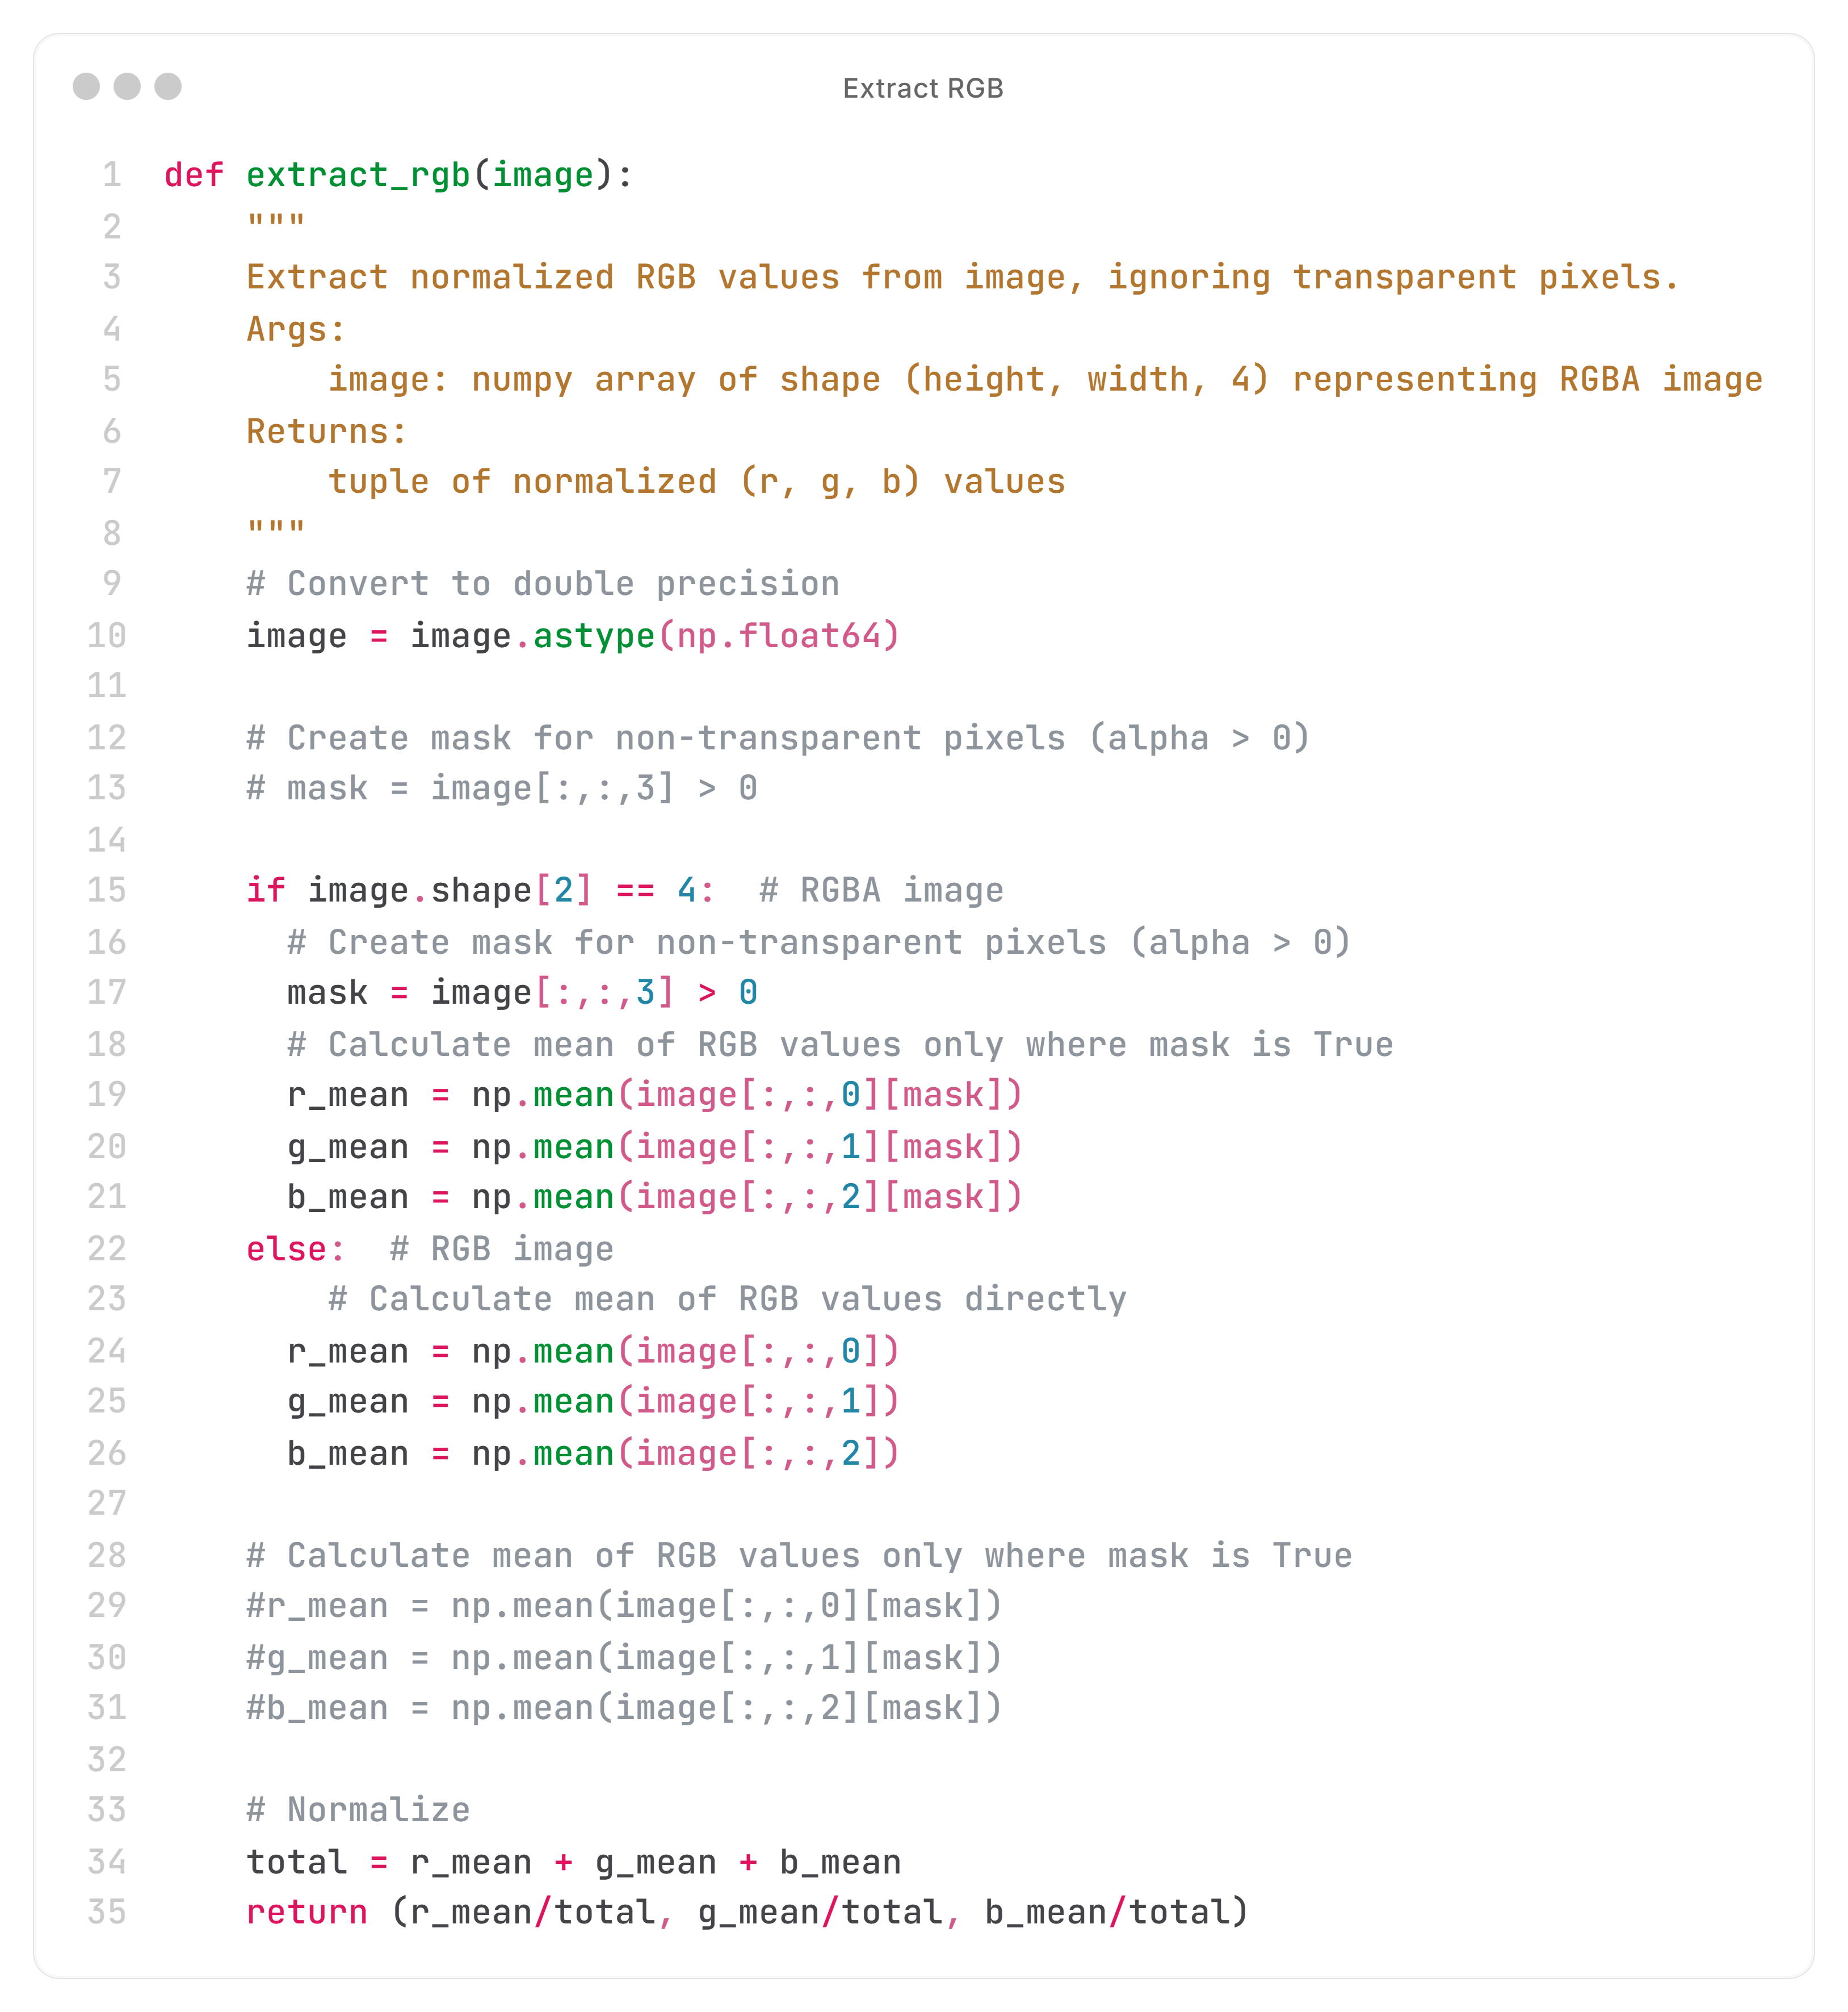
\includegraphics[width=0.6\textwidth]{figure/chapter-4-extract_rgb.png}
  \caption{Contoh hasil ekstraksi fitur warna RGB}
  \label{fig:extract_rgb}
\end{figure}

{Ekstraksi Fitur Warna RGB}
Fungsi ini mengekstrak rata-rata nilai RGB dari citra daun. Jika citra memiliki channel alpha (RGBA), fungsi hanya menghitung nilai RGB dari area yang tidak transparan — dengan kata lain, hanya dari bagian daun yang merupakan \textit{Region of Interest} (ROI). Setelah rata-rata tiap channel warna didapatkan, dilakukan normalisasi dengan membagi masing-masing nilai dengan jumlah total ketiga channel tersebut. Hasil akhirnya adalah nilai RGB terstandarisasi yang merepresentasikan distribusi warna utama dari citra daun.

\begin{figure}[H]
  \centering
  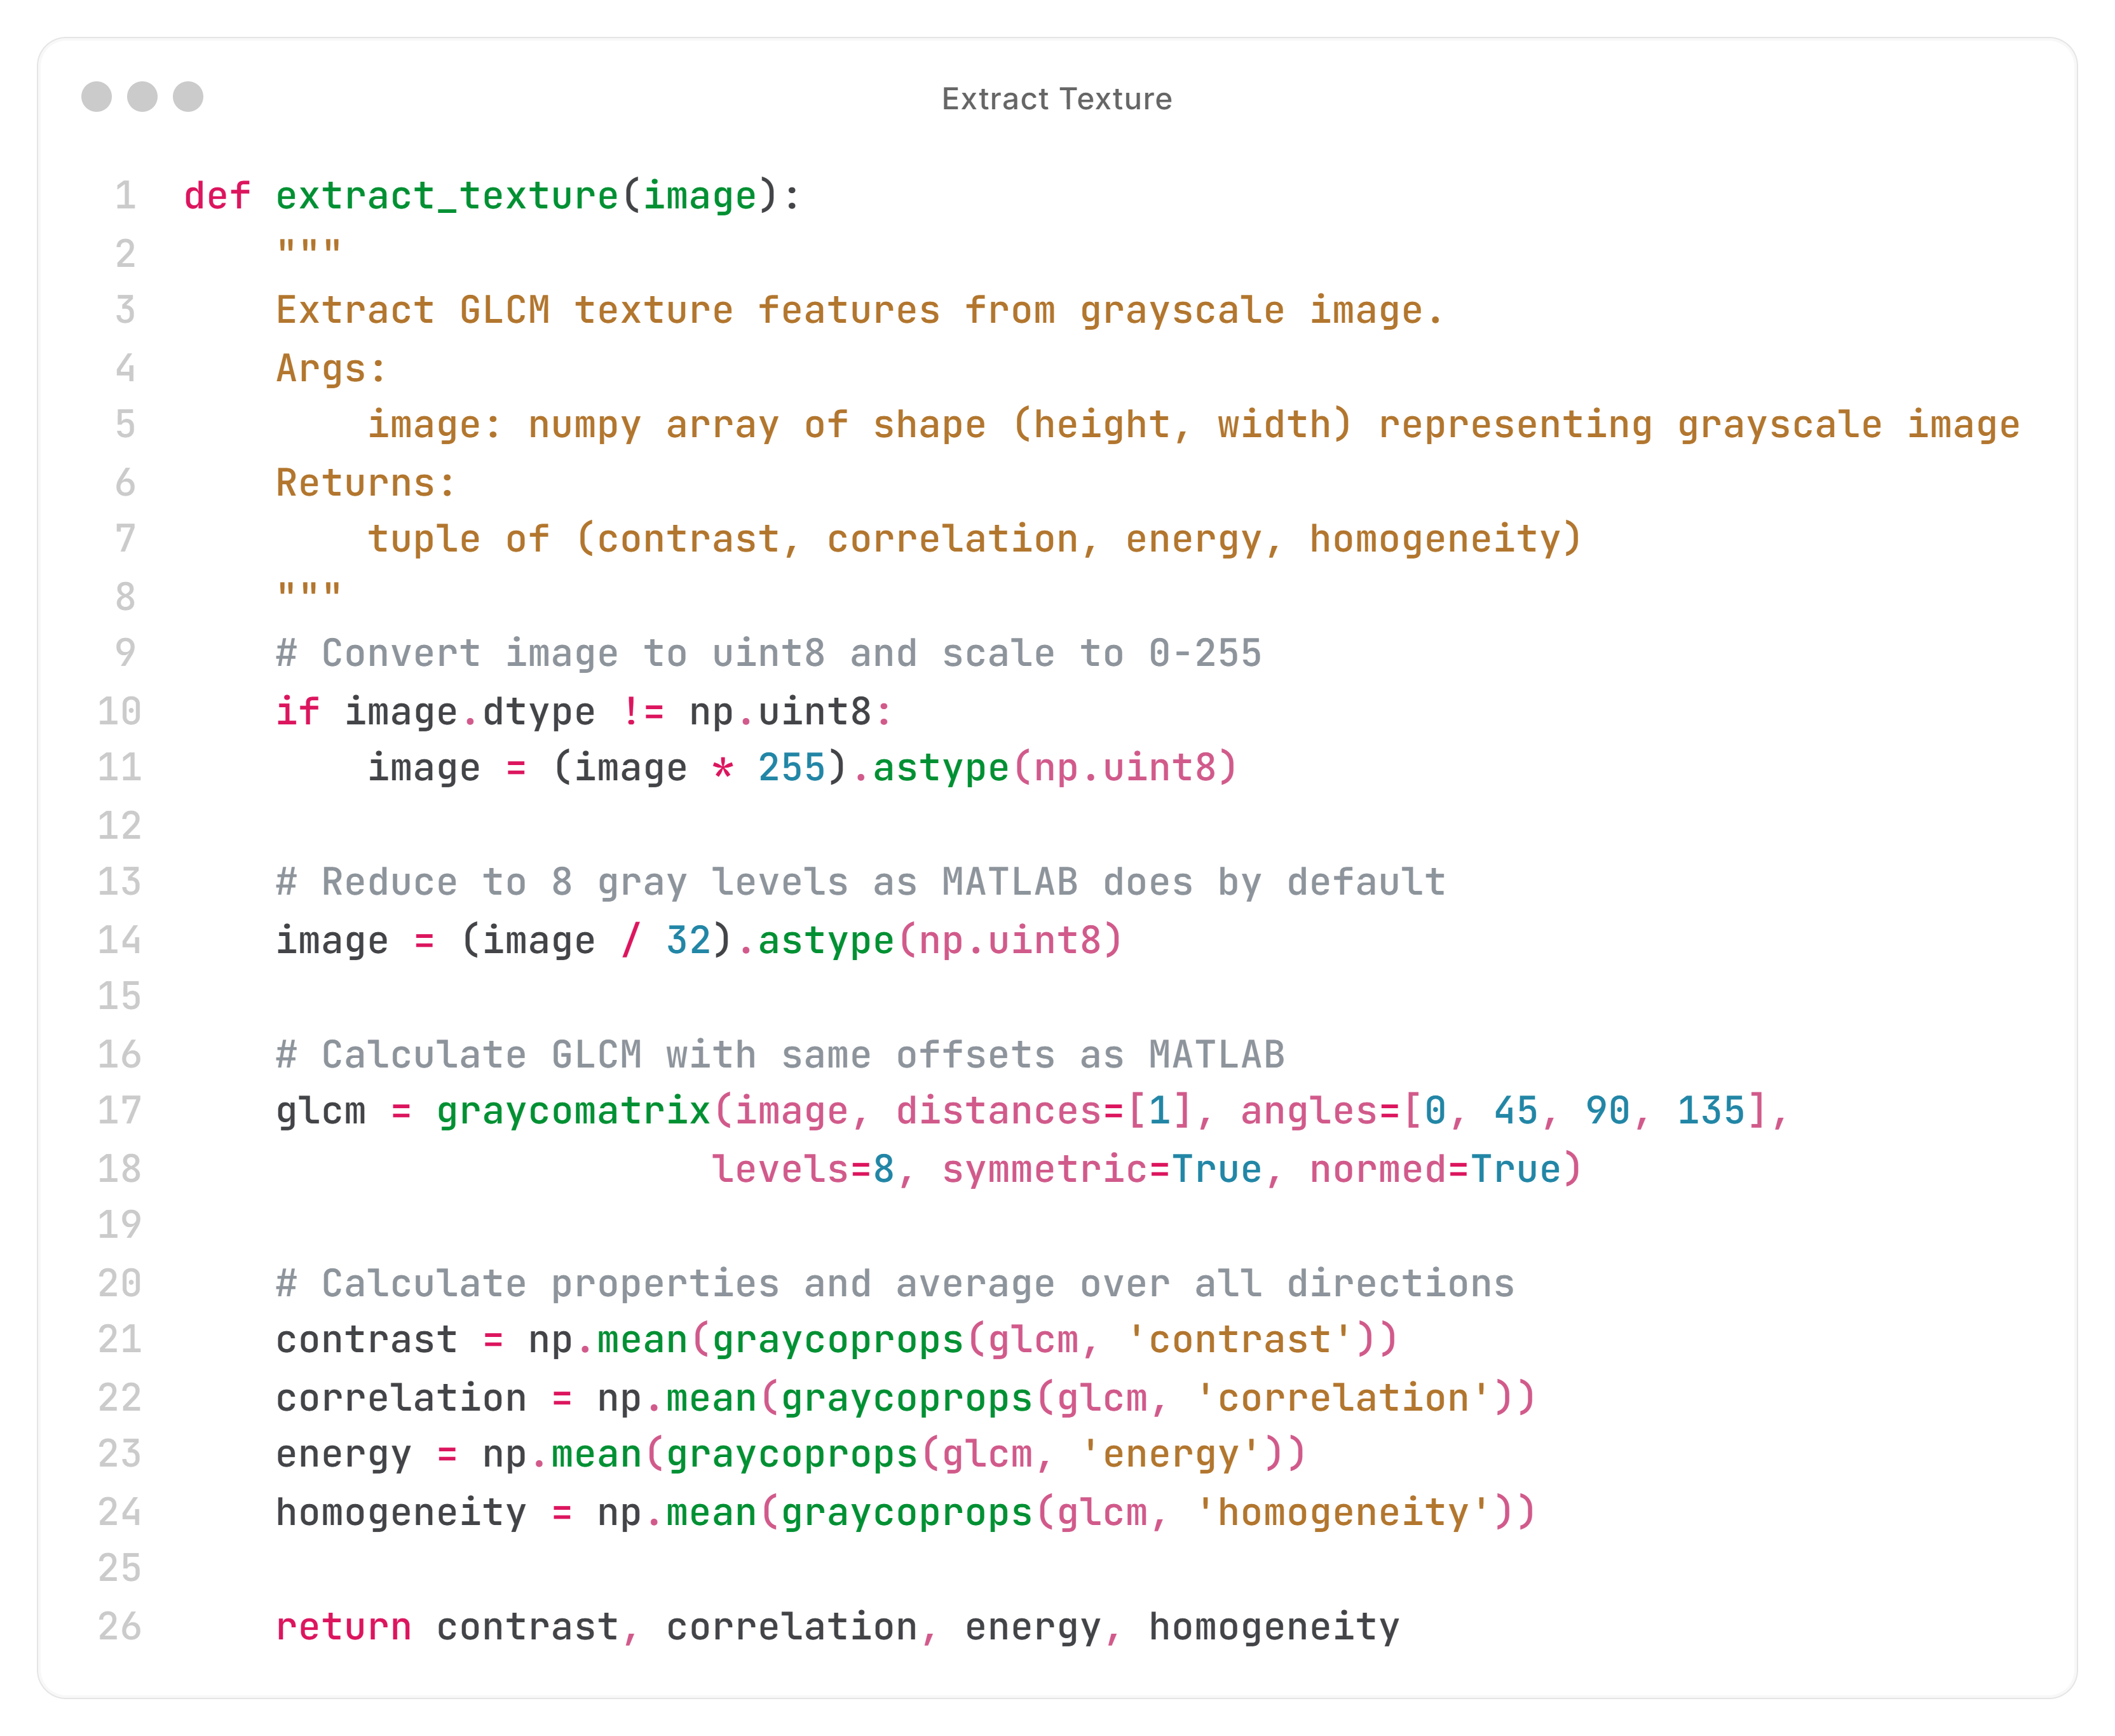
\includegraphics[width=0.6\textwidth]{figure/chapter-4-extract_texture.png}
  \caption{Contoh hasil ekstraksi tekstur}
  \label{fig:extract_rgb}
\end{figure}

{Ekstraksi Fitur Tekstur (GLCM)}
Fungsi ini mengekstrak fitur tekstur dari citra grayscale dengan menggunakan metode \textit{Gray Level Co-Occurrence Matrix} (GLCM). Citra terlebih dahulu dikonversi menjadi 8 tingkat keabuan (\textit{gray level}) untuk menyederhanakan informasi tekstur. GLCM dihitung pada empat arah sudut (0\textdegree, 45\textdegree, 90\textdegree, dan 135\textdegree) dengan jarak 1 piksel. Selanjutnya, empat properti tekstur utama dihitung dari GLCM, yaitu kontras, korelasi, energi, dan homogenitas. Nilai dari masing-masing properti kemudian dirata-ratakan dari seluruh arah sudut untuk menghasilkan representasi tekstur yang lebih stabil.

\subsection{Memproses Gambar Daun menjadi Kerangka Data} \label{IV.Memproses Gambar Daun menjadi Kerangka Data}

\begin{figure}[H]
  \centering
  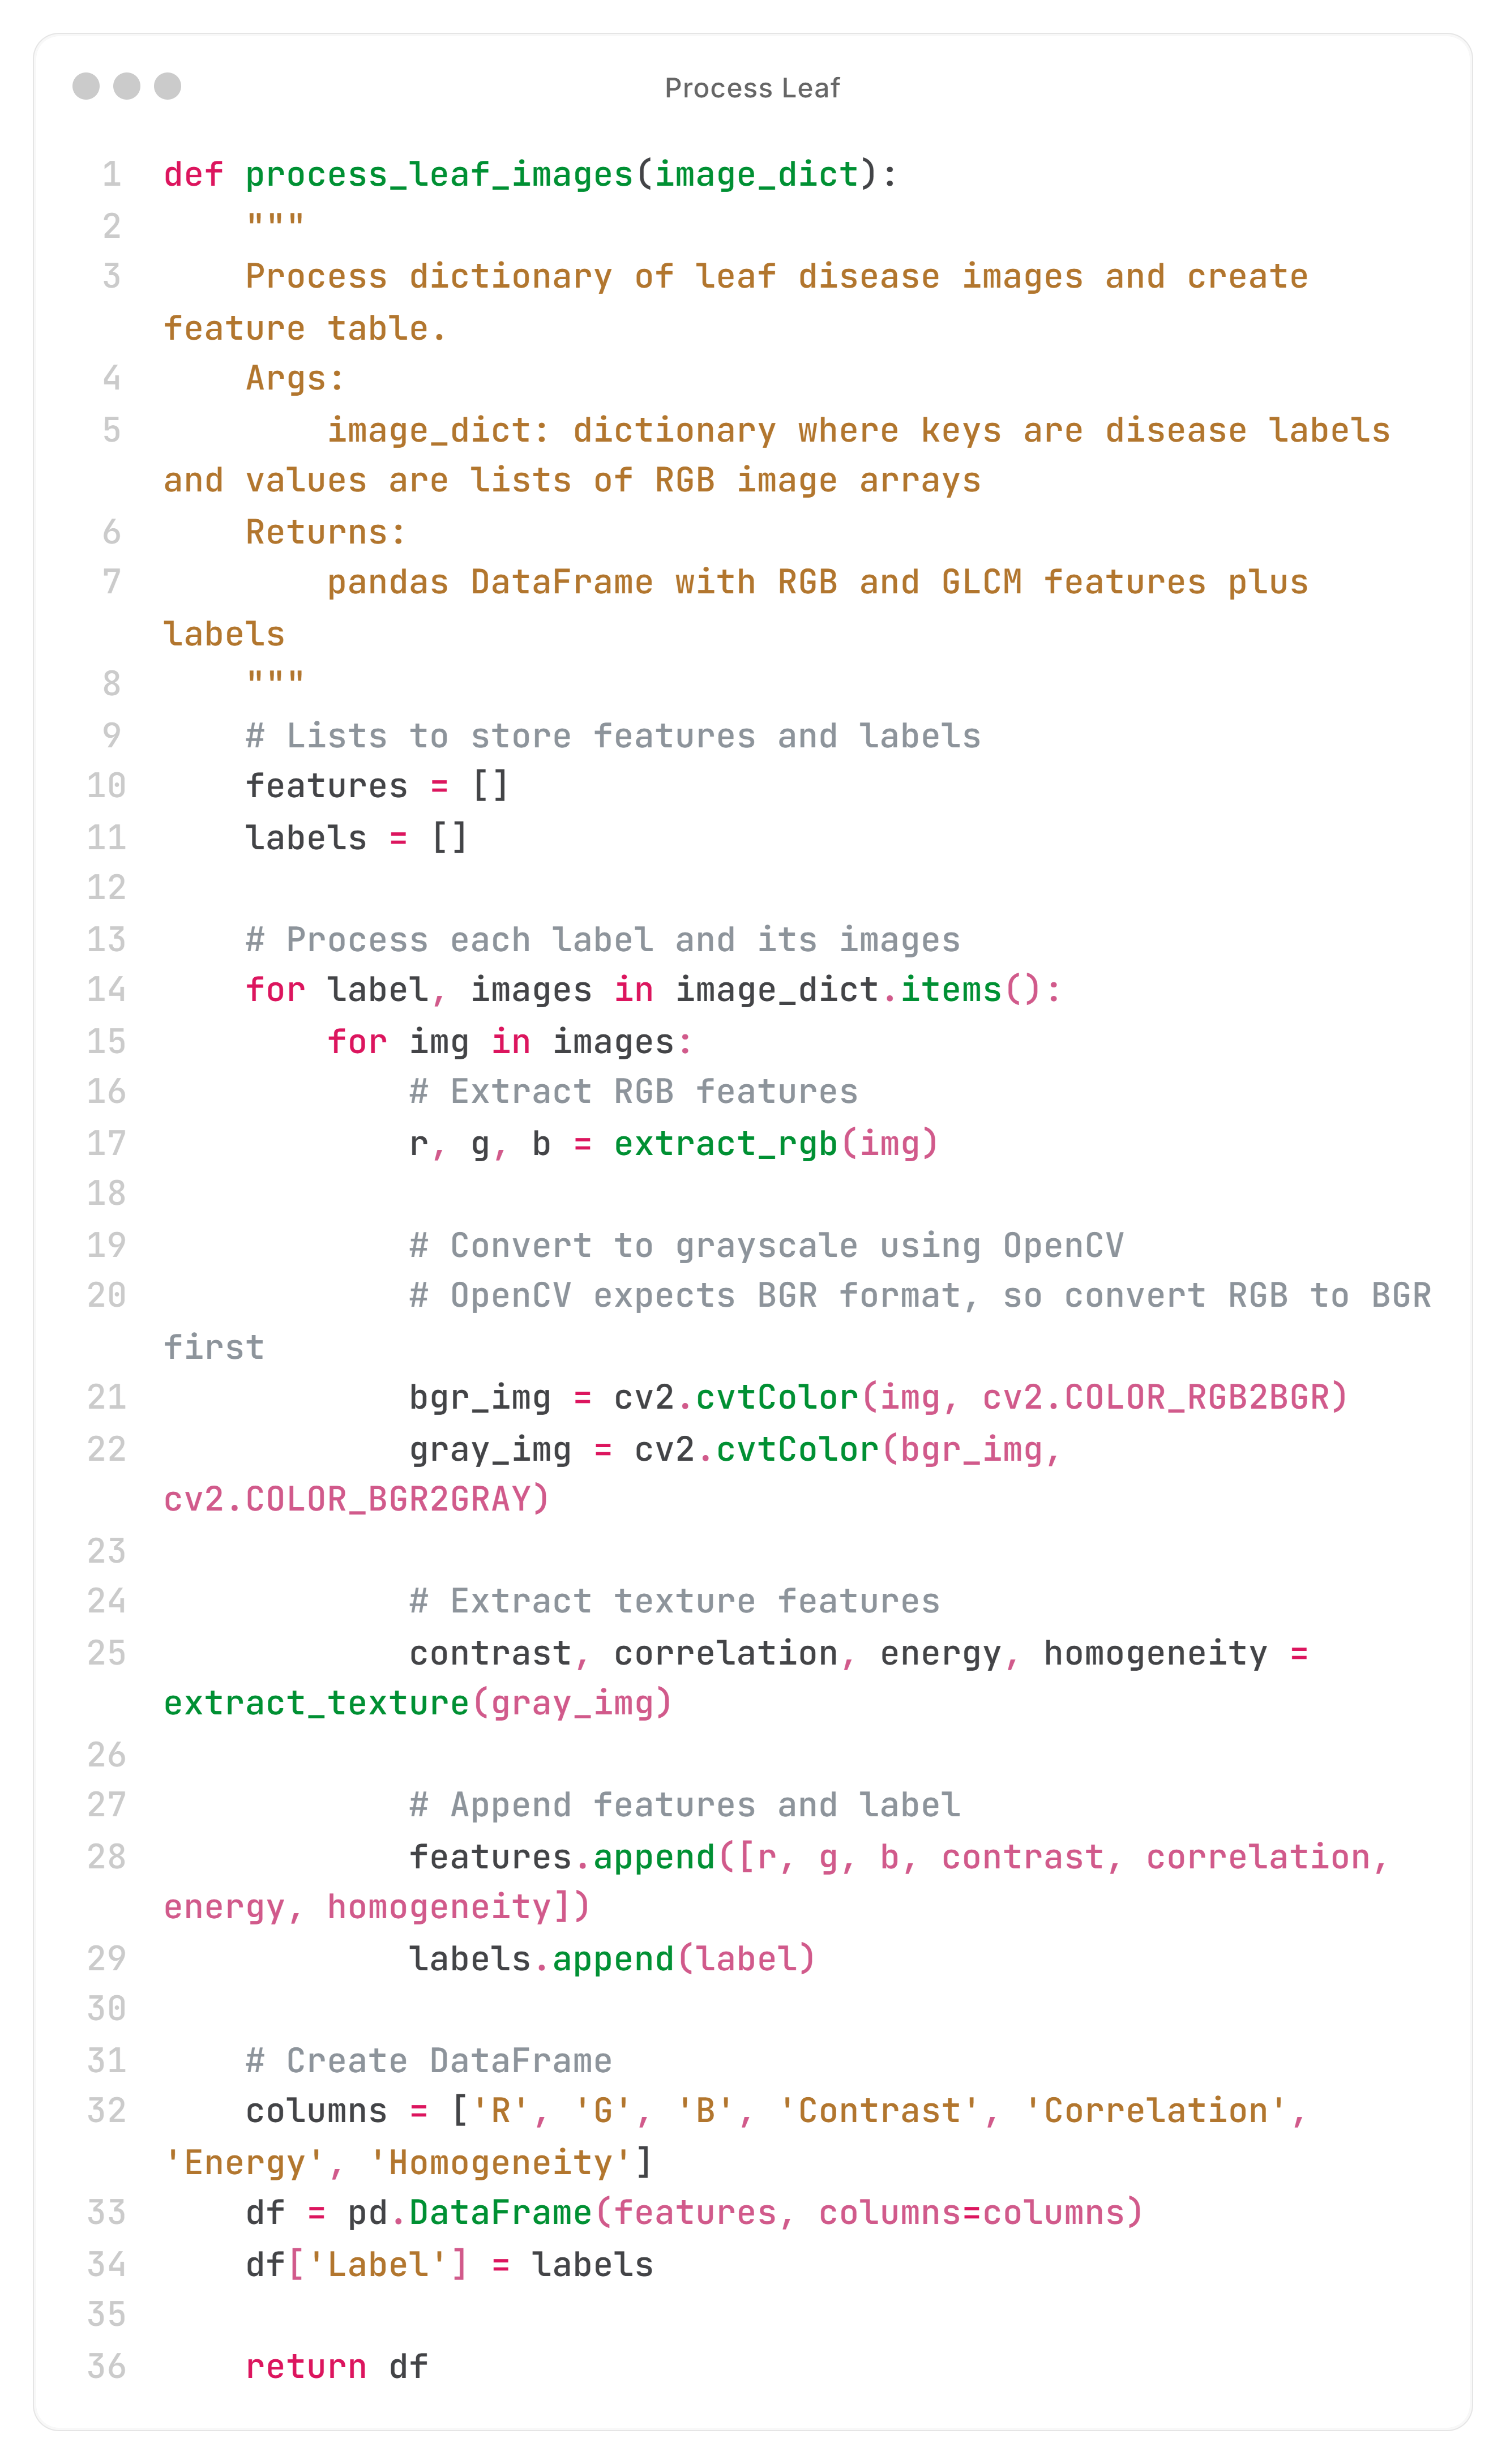
\includegraphics[width=0.6\textwidth]{figure/chapter-4-process_leaf.png}
  \caption{Contoh hasil pemrosesan gambar daun menjadi kerangka data}
  \label{fig:extract_rgb}
\end{figure}

Fungsi ini mengelola keseluruhan proses ekstraksi fitur dari dataset citra daun. Fungsi menerima sebuah \textit{dictionary} dengan label penyakit sebagai \textit{key} dan daftar citra RGB sebagai \textit{value}. Untuk setiap citra, fitur warna RGB dan fitur tekstur GLCM diekstrak, kemudian disimpan bersama labelnya dalam sebuah tabel (\textit{DataFrame}). 

Tabel ini memiliki kolom sebagai berikut: \textbf{R}, \textbf{G}, \textbf{B}, \textbf{Contrast}, \textbf{Correlation}, \textbf{Energy}, \textbf{Homogeneity}, dan \textbf{Label}. Hasil akhirnya berupa \textit{DataFrame} yang siap digunakan sebagai input untuk pelatihan model.

\subsection{Pembagian Dataset} \label{IV.Pembagian Dataset}

Setelah melalui proses ekstraksi, dataset yang diperoleh kemudian dibagi menjadi dua bagian: \textit{data training} dan \textit{data testing}. Rasio pembagian yang digunakan adalah 80:20, di mana 80\% dari total data digunakan untuk melatih model, dan 20\% sisanya digunakan untuk menguji performa model terhadap data yang belum pernah ``dilihat'' oleh model sebelumnya.

Berikut adalah kode yang digunakan untuk melakukan proses pembagian tersebut:

\begin{figure}[H]
  \centering
  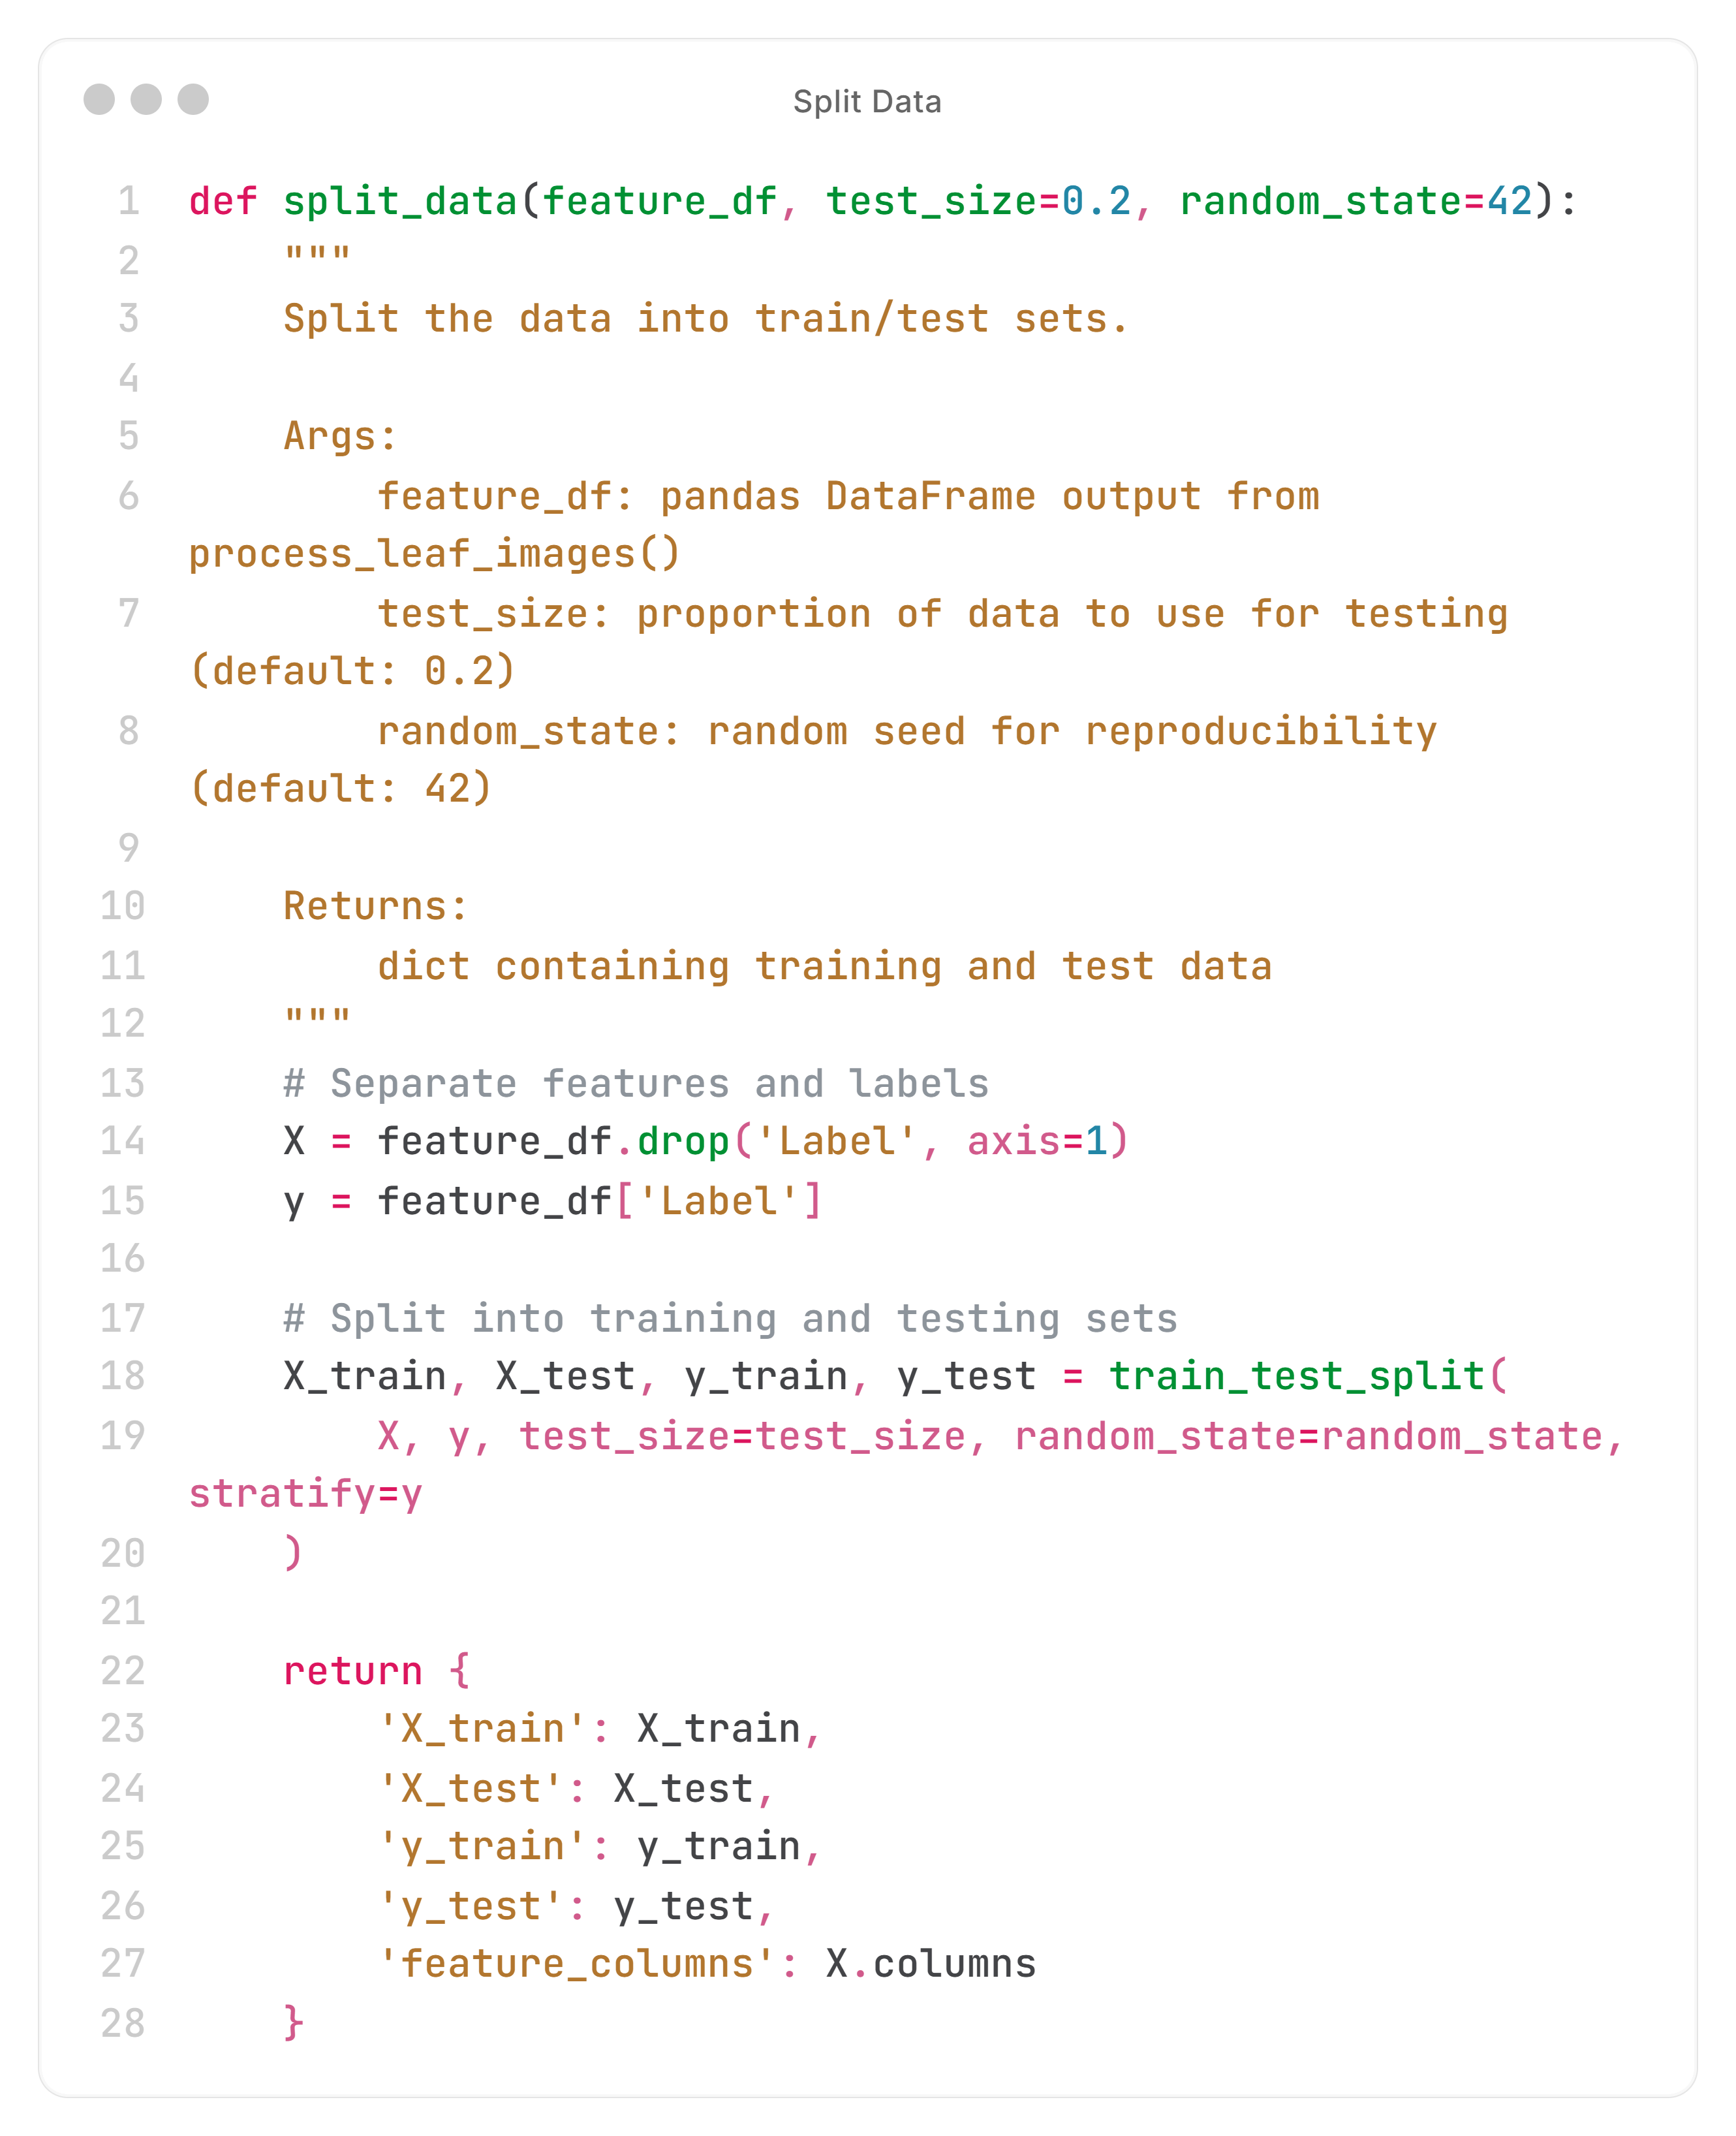
\includegraphics[width=0.6\textwidth]{figure/chapter-4-split_data.png}
  \caption{Contoh hasil pembagian dataset menjadi data training dan testing}
  \label{fig:extract_rgb}
\end{figure}

% Tabel ini memiliki kolom sebagai berikut: \textbf{R}, \textbf{G}, \textbf{B}, \textbf{Contrast}, \textbf{Correlation}, \textbf{Energy}, \textbf{Homogeneity}, dan \textbf{Label}.


\subsection{Pembuatan Model} \label{IV.Pembuatan Model}
Pada tahap ini, dilakukan pembuatan tiga jenis model machine learning berbasis algoritma \textit{Gaussian Naive Bayes}. Masing-masing model dibangun dengan pendekatan berbeda.

\subsection{Original Naive Bayes} \label{IV.Original Naïve Bayes}
Model ini menggunakan fitur yang diperoleh secara langsung tanpa melalui proses optimasi atau seleksi fitur lanjutan. Tujuan dari model ini adalah untuk membandingkan performa dasar algoritma \textit{Naive Bayes} sebelum dilakukan peningkatan dengan algoritma optimasi.

\begin{figure}[H]
  \centering
  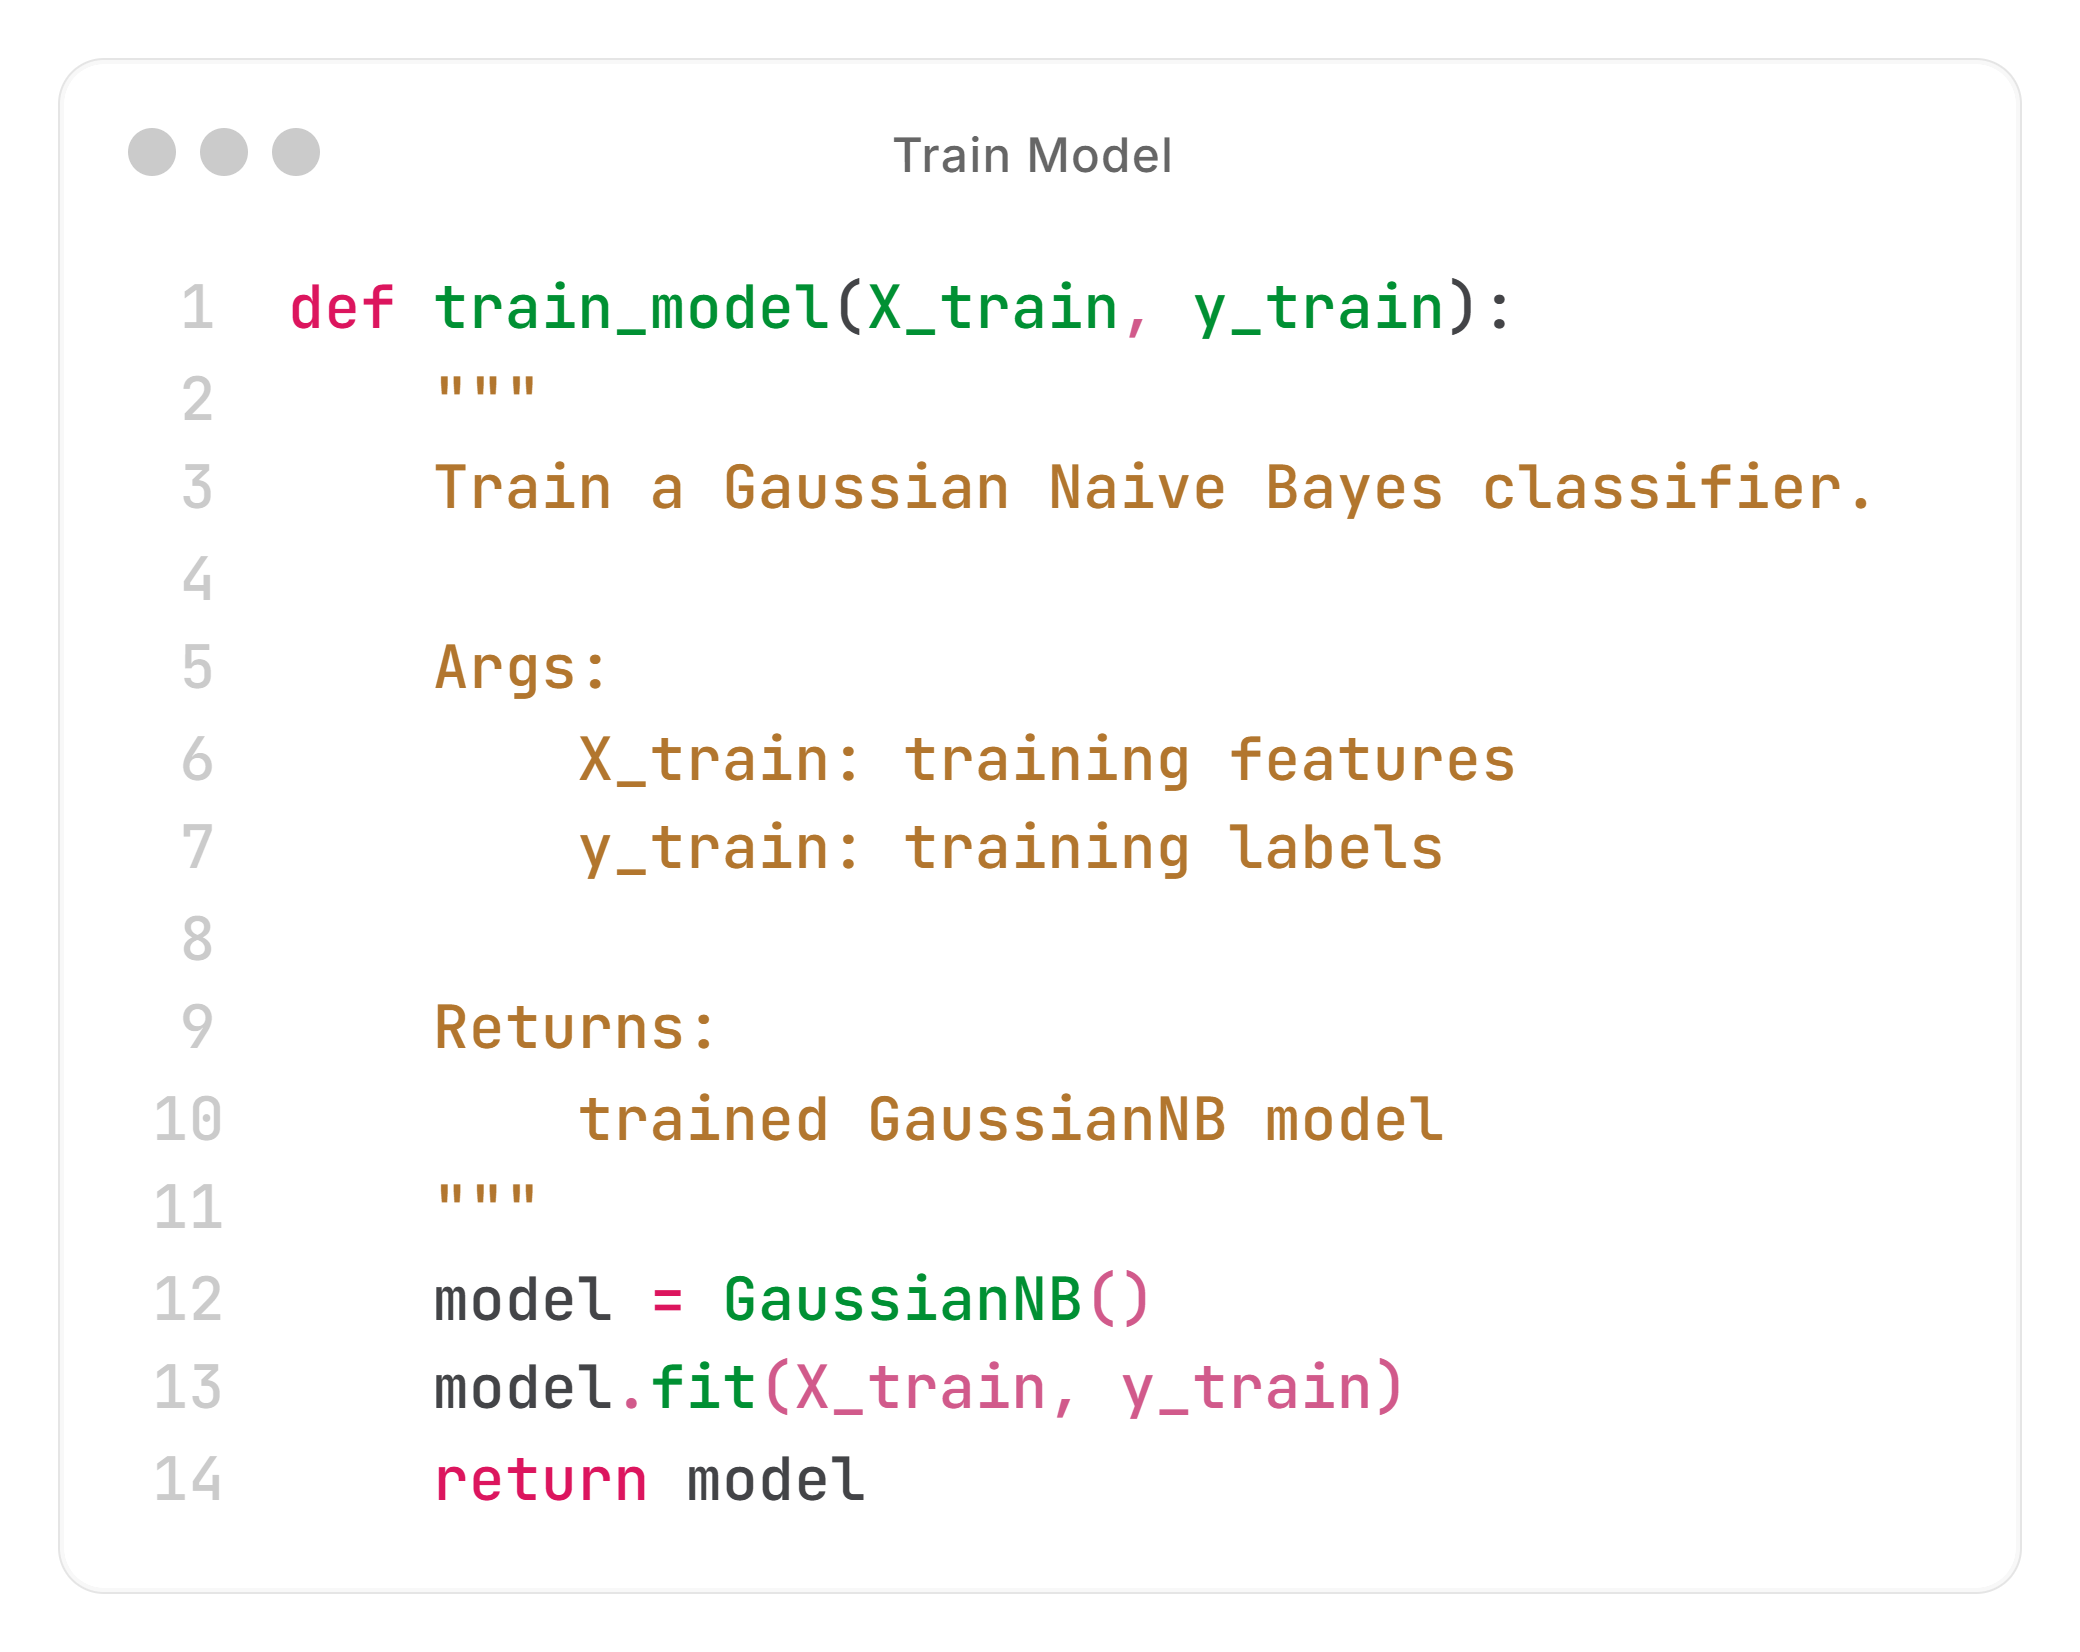
\includegraphics[width=0.6\textwidth]{figure/chapter-4-train_model.png}
  \caption{Contoh hasil ekstraksi tekstur}
  \label{fig:extract_rgb}
\end{figure}

Model ini menggunakan parameter default dari \textit{GaussianNB} tanpa melakukan tuning. Cocok digunakan sebagai \textit{baseline} untuk dibandingkan dengan model yang telah dioptimasi.


\subsection{GA Optimized Naive Bayes} \label{IV.GA Optimized Naive Bayes}
Model ini menggunakan pendekatan algoritma \textit{Genetic Algorithm (GA)} untuk melakukan seleksi fitur yang paling relevan terhadap klasifikasi. Dengan mengoptimasi subset fitur, model diharapkan dapat meningkatkan akurasi klasifikasi dibandingkan model dasar. Algoritma GA bekerja berdasarkan prinsip evolusi biologis, seperti seleksi alam dan genetika, untuk menemukan kombinasi fitur terbaik.

\begin{figure}[H]
  \centering
  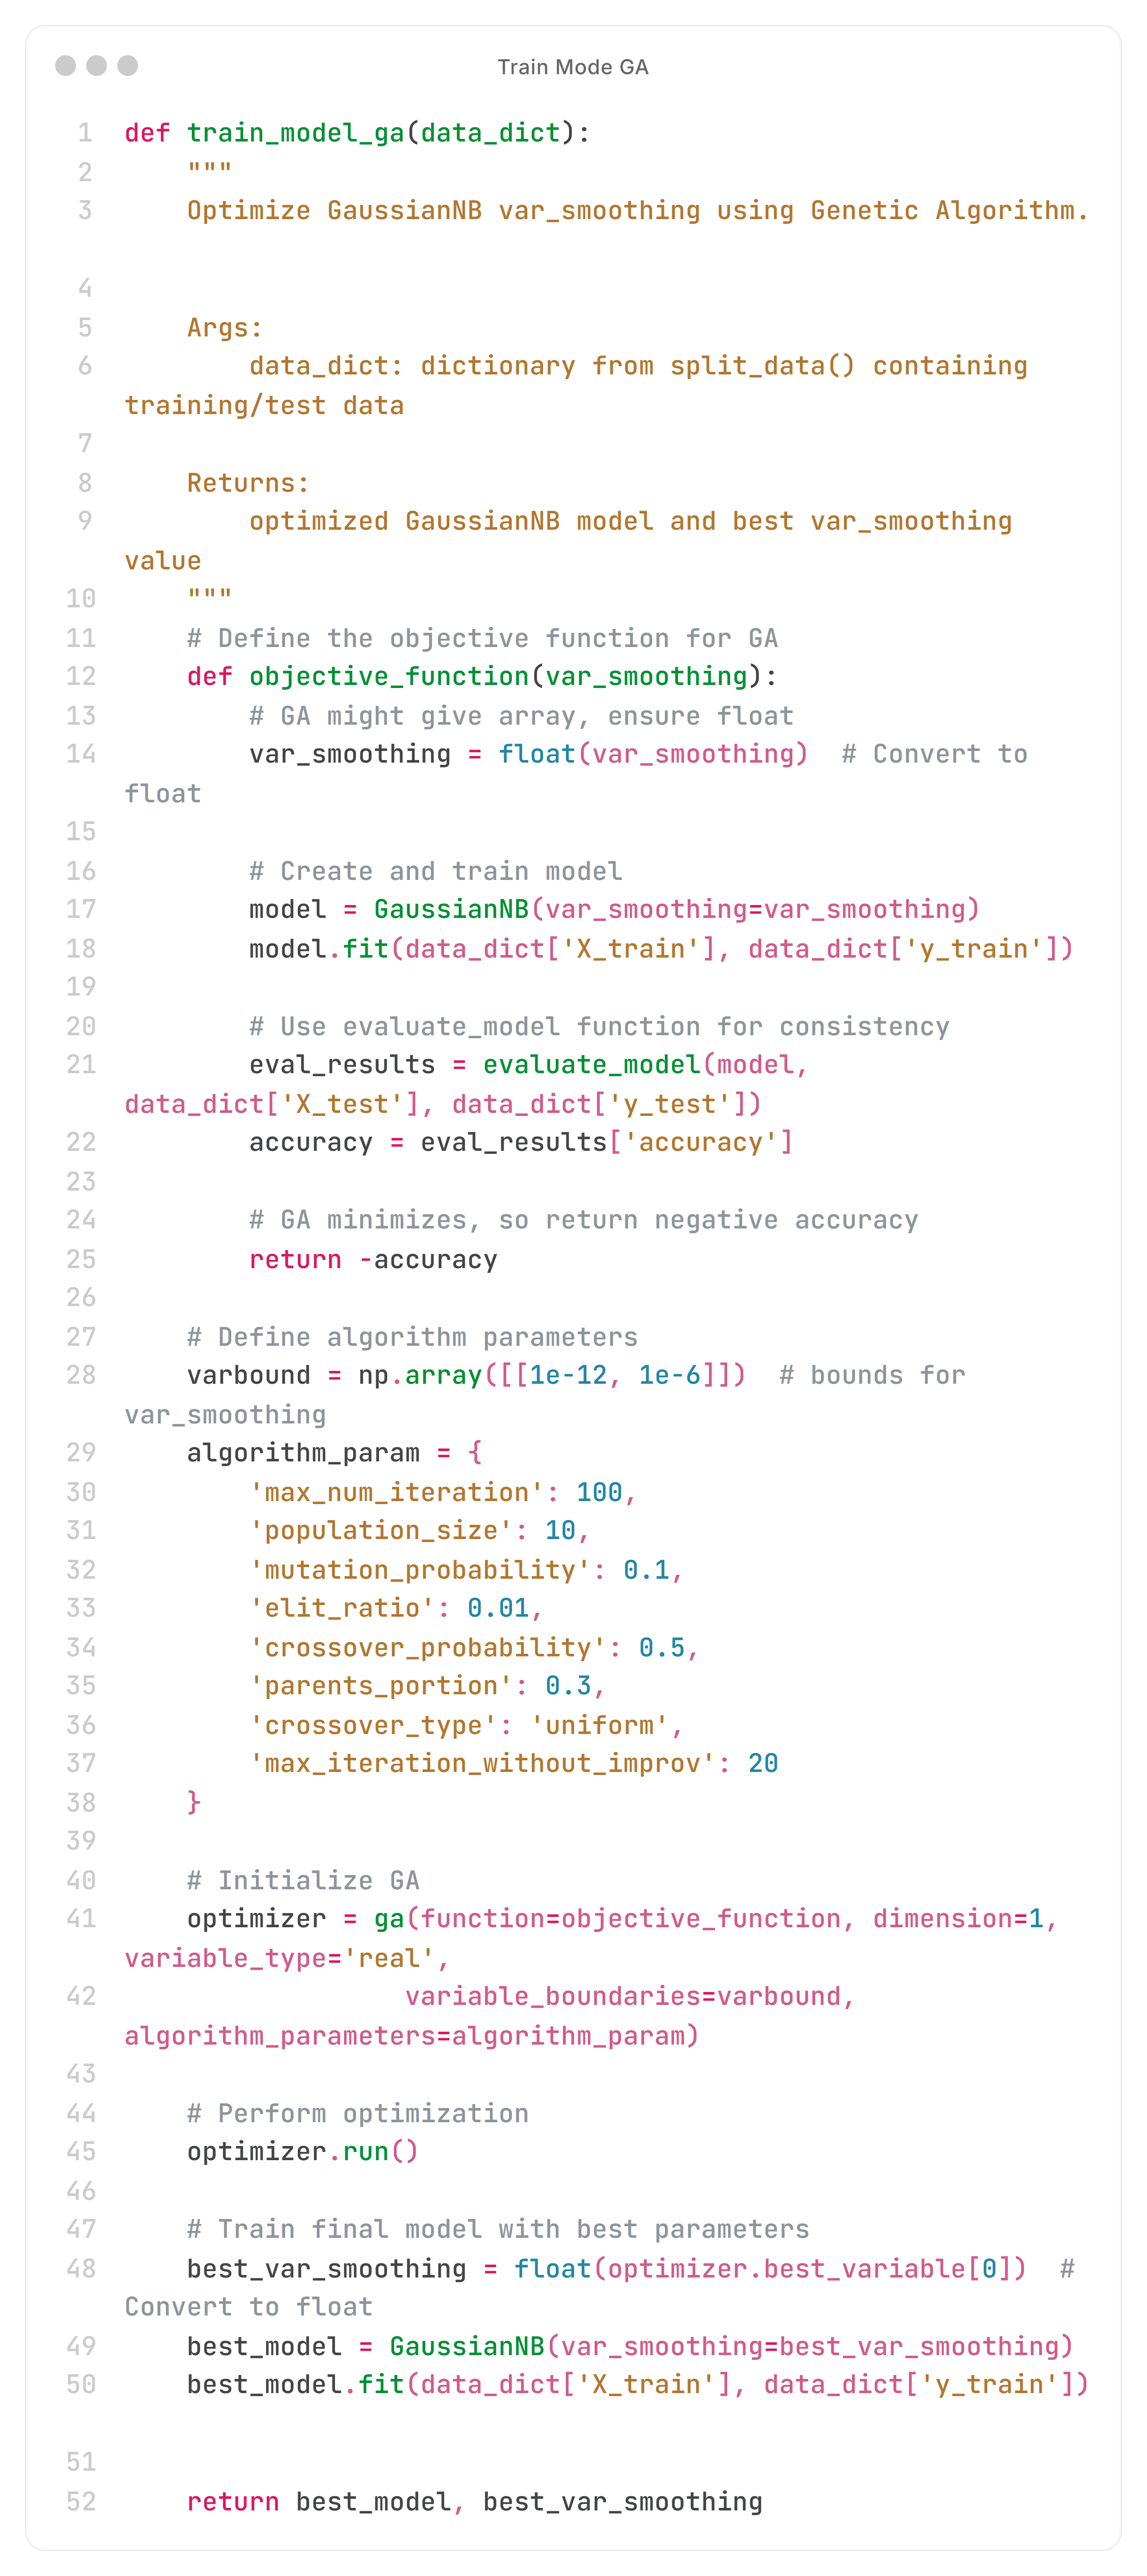
\includegraphics[width=0.6\textwidth]{figure/chapter-4-train_model_ga.png}
  \caption{Contoh hasil training model dengan GA}
  \label{fig:extract_rgb}
\end{figure}

Model ini menggunakan algoritma \textit{Genetic Algorithm (GA)} untuk menemukan nilai terbaik dari hyperparameter \texttt{var\_smoothing}, yang dapat meningkatkan akurasi klasifikasi.

\begin{figure}[H]
  \centering
  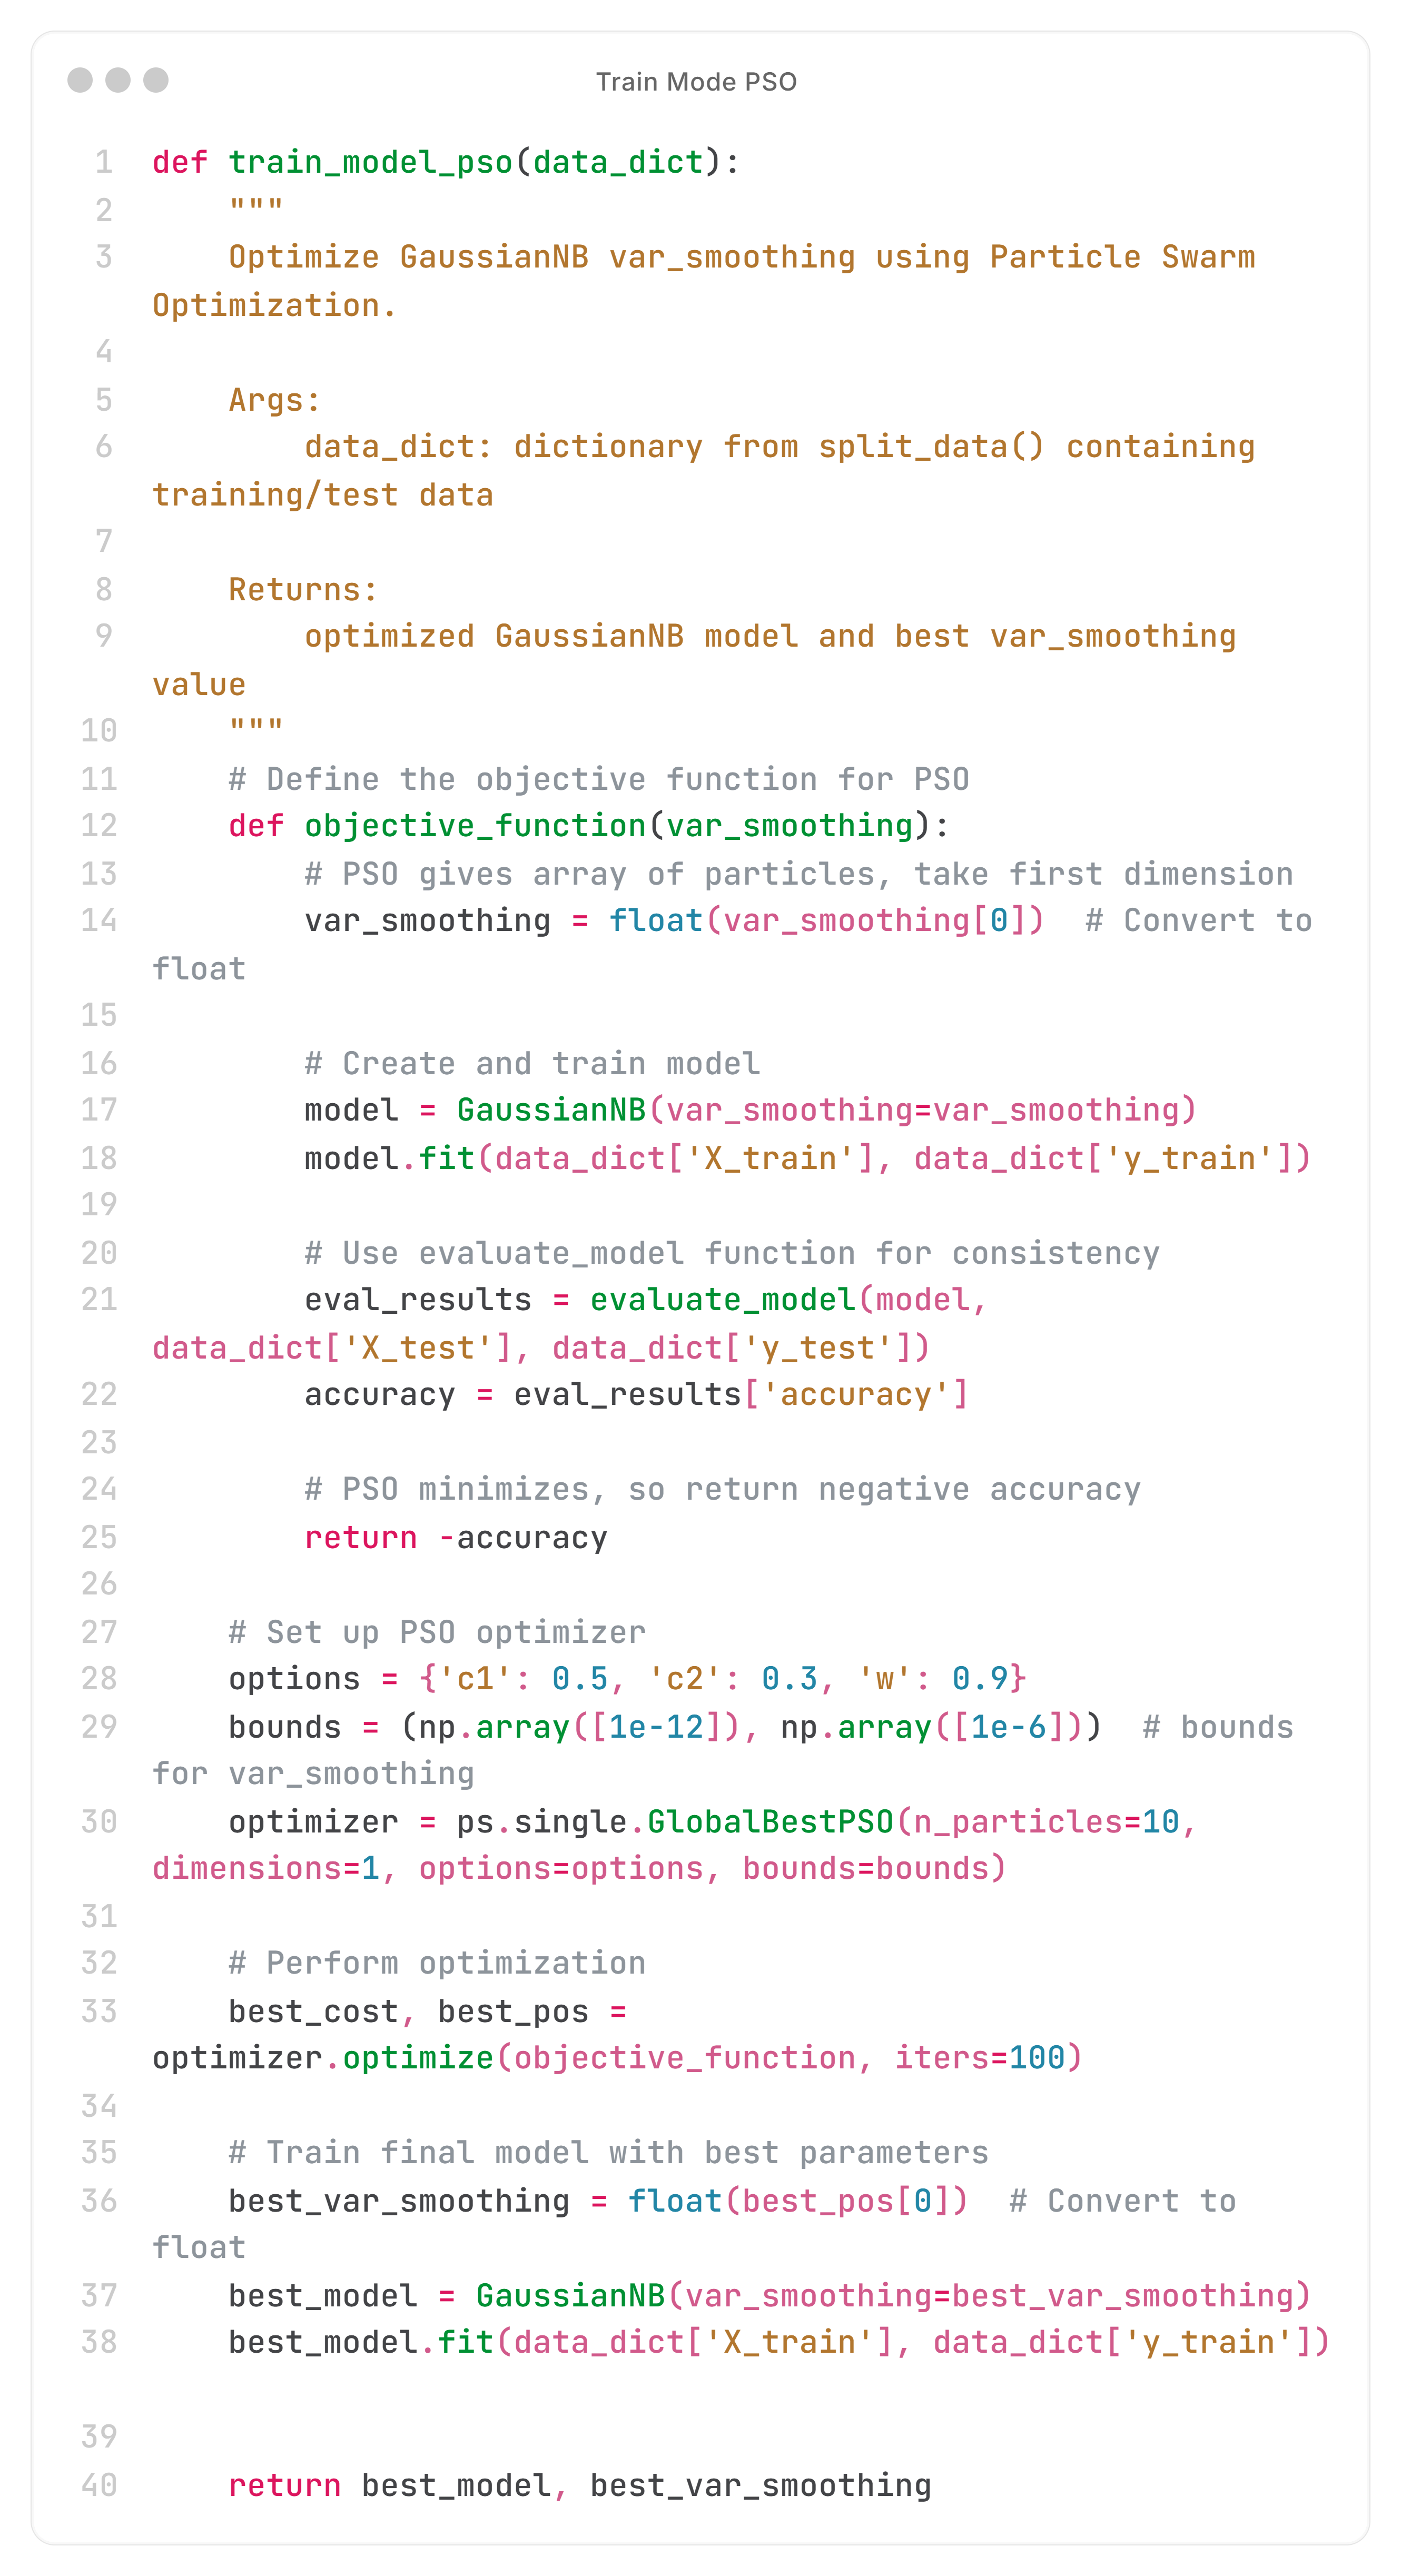
\includegraphics[width=0.6\textwidth]{figure/chapter-4-train_model_pso.png}
  \caption{Contoh training model dengan PSO}
  \label{fig:extract_rgb}
\end{figure}

Model ini menggunakan algoritma \textit{Particle Swarm Optimization (PSO)} yang bekerja dengan mensimulasikan pergerakan partikel dalam ruang solusi. Setiap partikel mewakili kemungkinan nilai \texttt{var\_smoothing}. Model dengan akurasi terbaik dipilih sebagai solusi optimal.

\subsection{Evaluasi} \label{IV.Evaluasi}
Setelah model dilatih, langkah selanjutnya adalah mengevaluasi performanya menggunakan metrik seperti akurasi, laporan klasifikasi, dan \textit{confusion matrix}.

\begin{figure}[H]
  \centering
  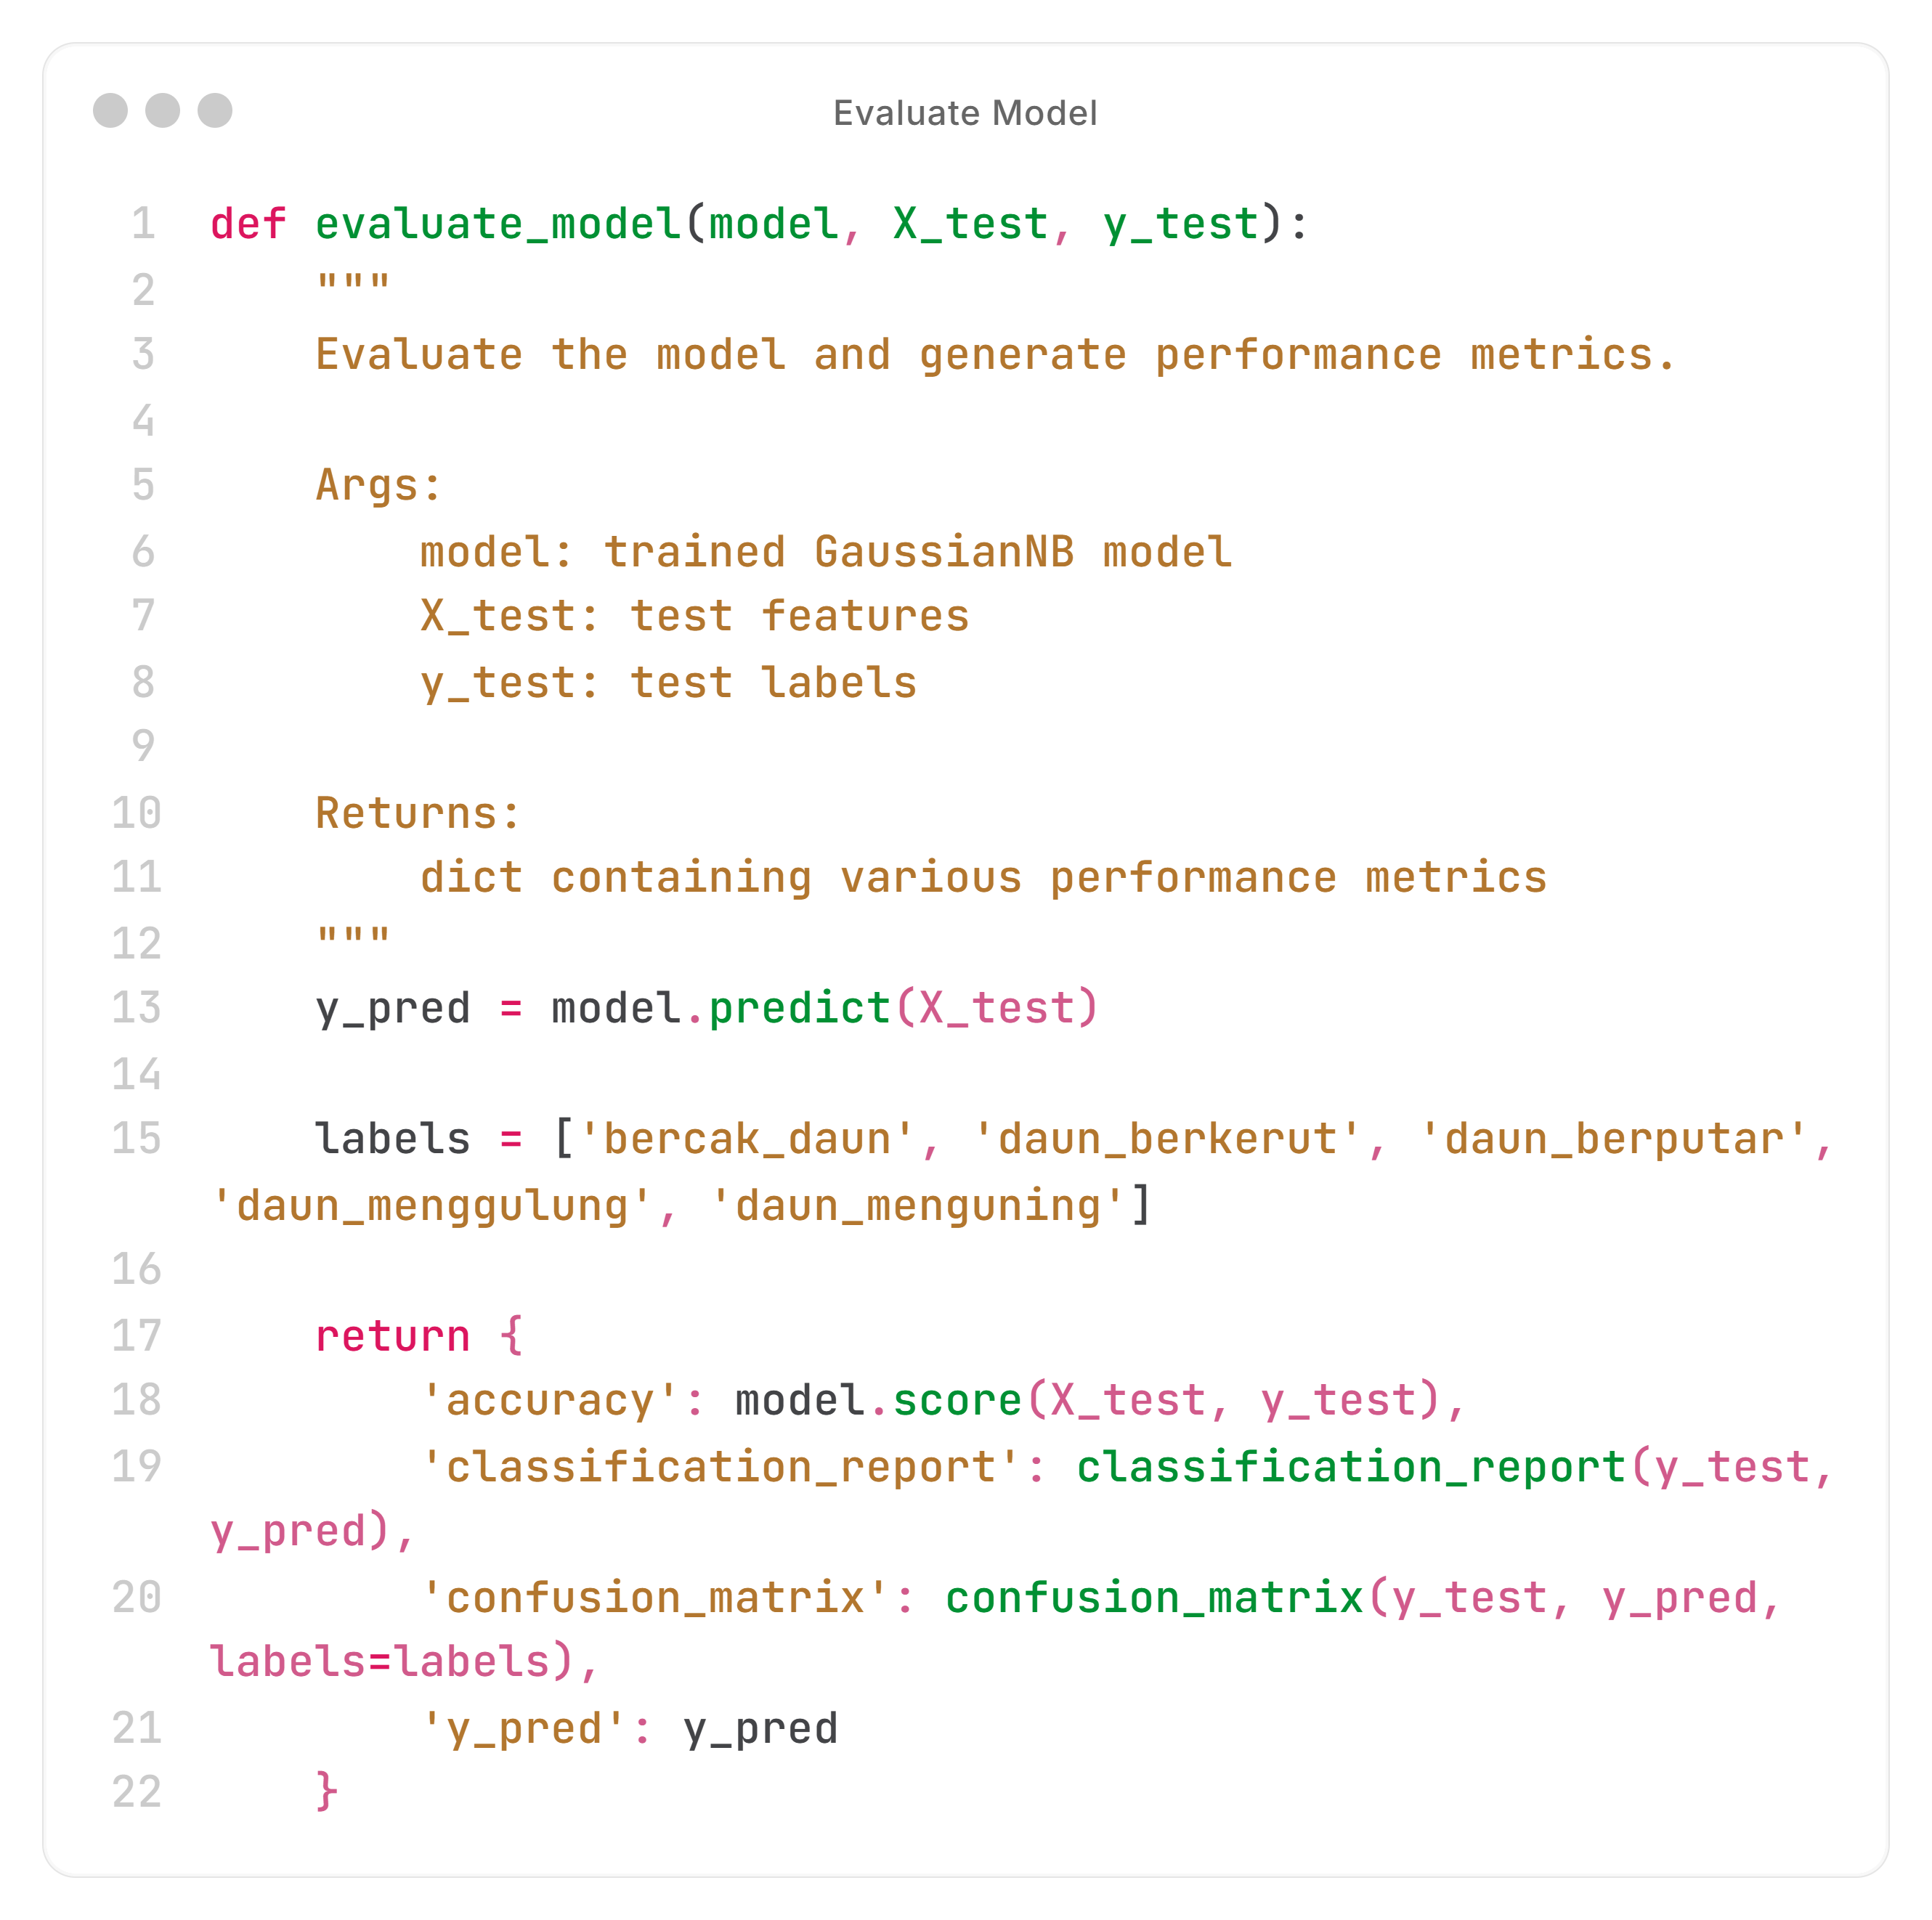
\includegraphics[width=0.6\textwidth]{figure/chapter-4-evaluasi.png}
  \caption{Contoh hasil evaluasi model}
  \label{fig:extract_rgb}
\end{figure}

Fungsi ini memberikan hasil evaluasi menyeluruh dari model, termasuk:
\begin{enumerate}
    \item {\textbf{Accuracy}: Persentase prediksi yang benar.}
    \item {\textbf{Classification Report}: Menampilkan metrik \textit{Precision}, \textit{Recall}, dan \textit{F1-score}.}
    \item {\textbf{Confusion Matrix}: Matriks yang membandingkan klasifikasi aktual dengan prediksi model.}
\end{enumerate}

\begin{figure}[H]
  \centering
  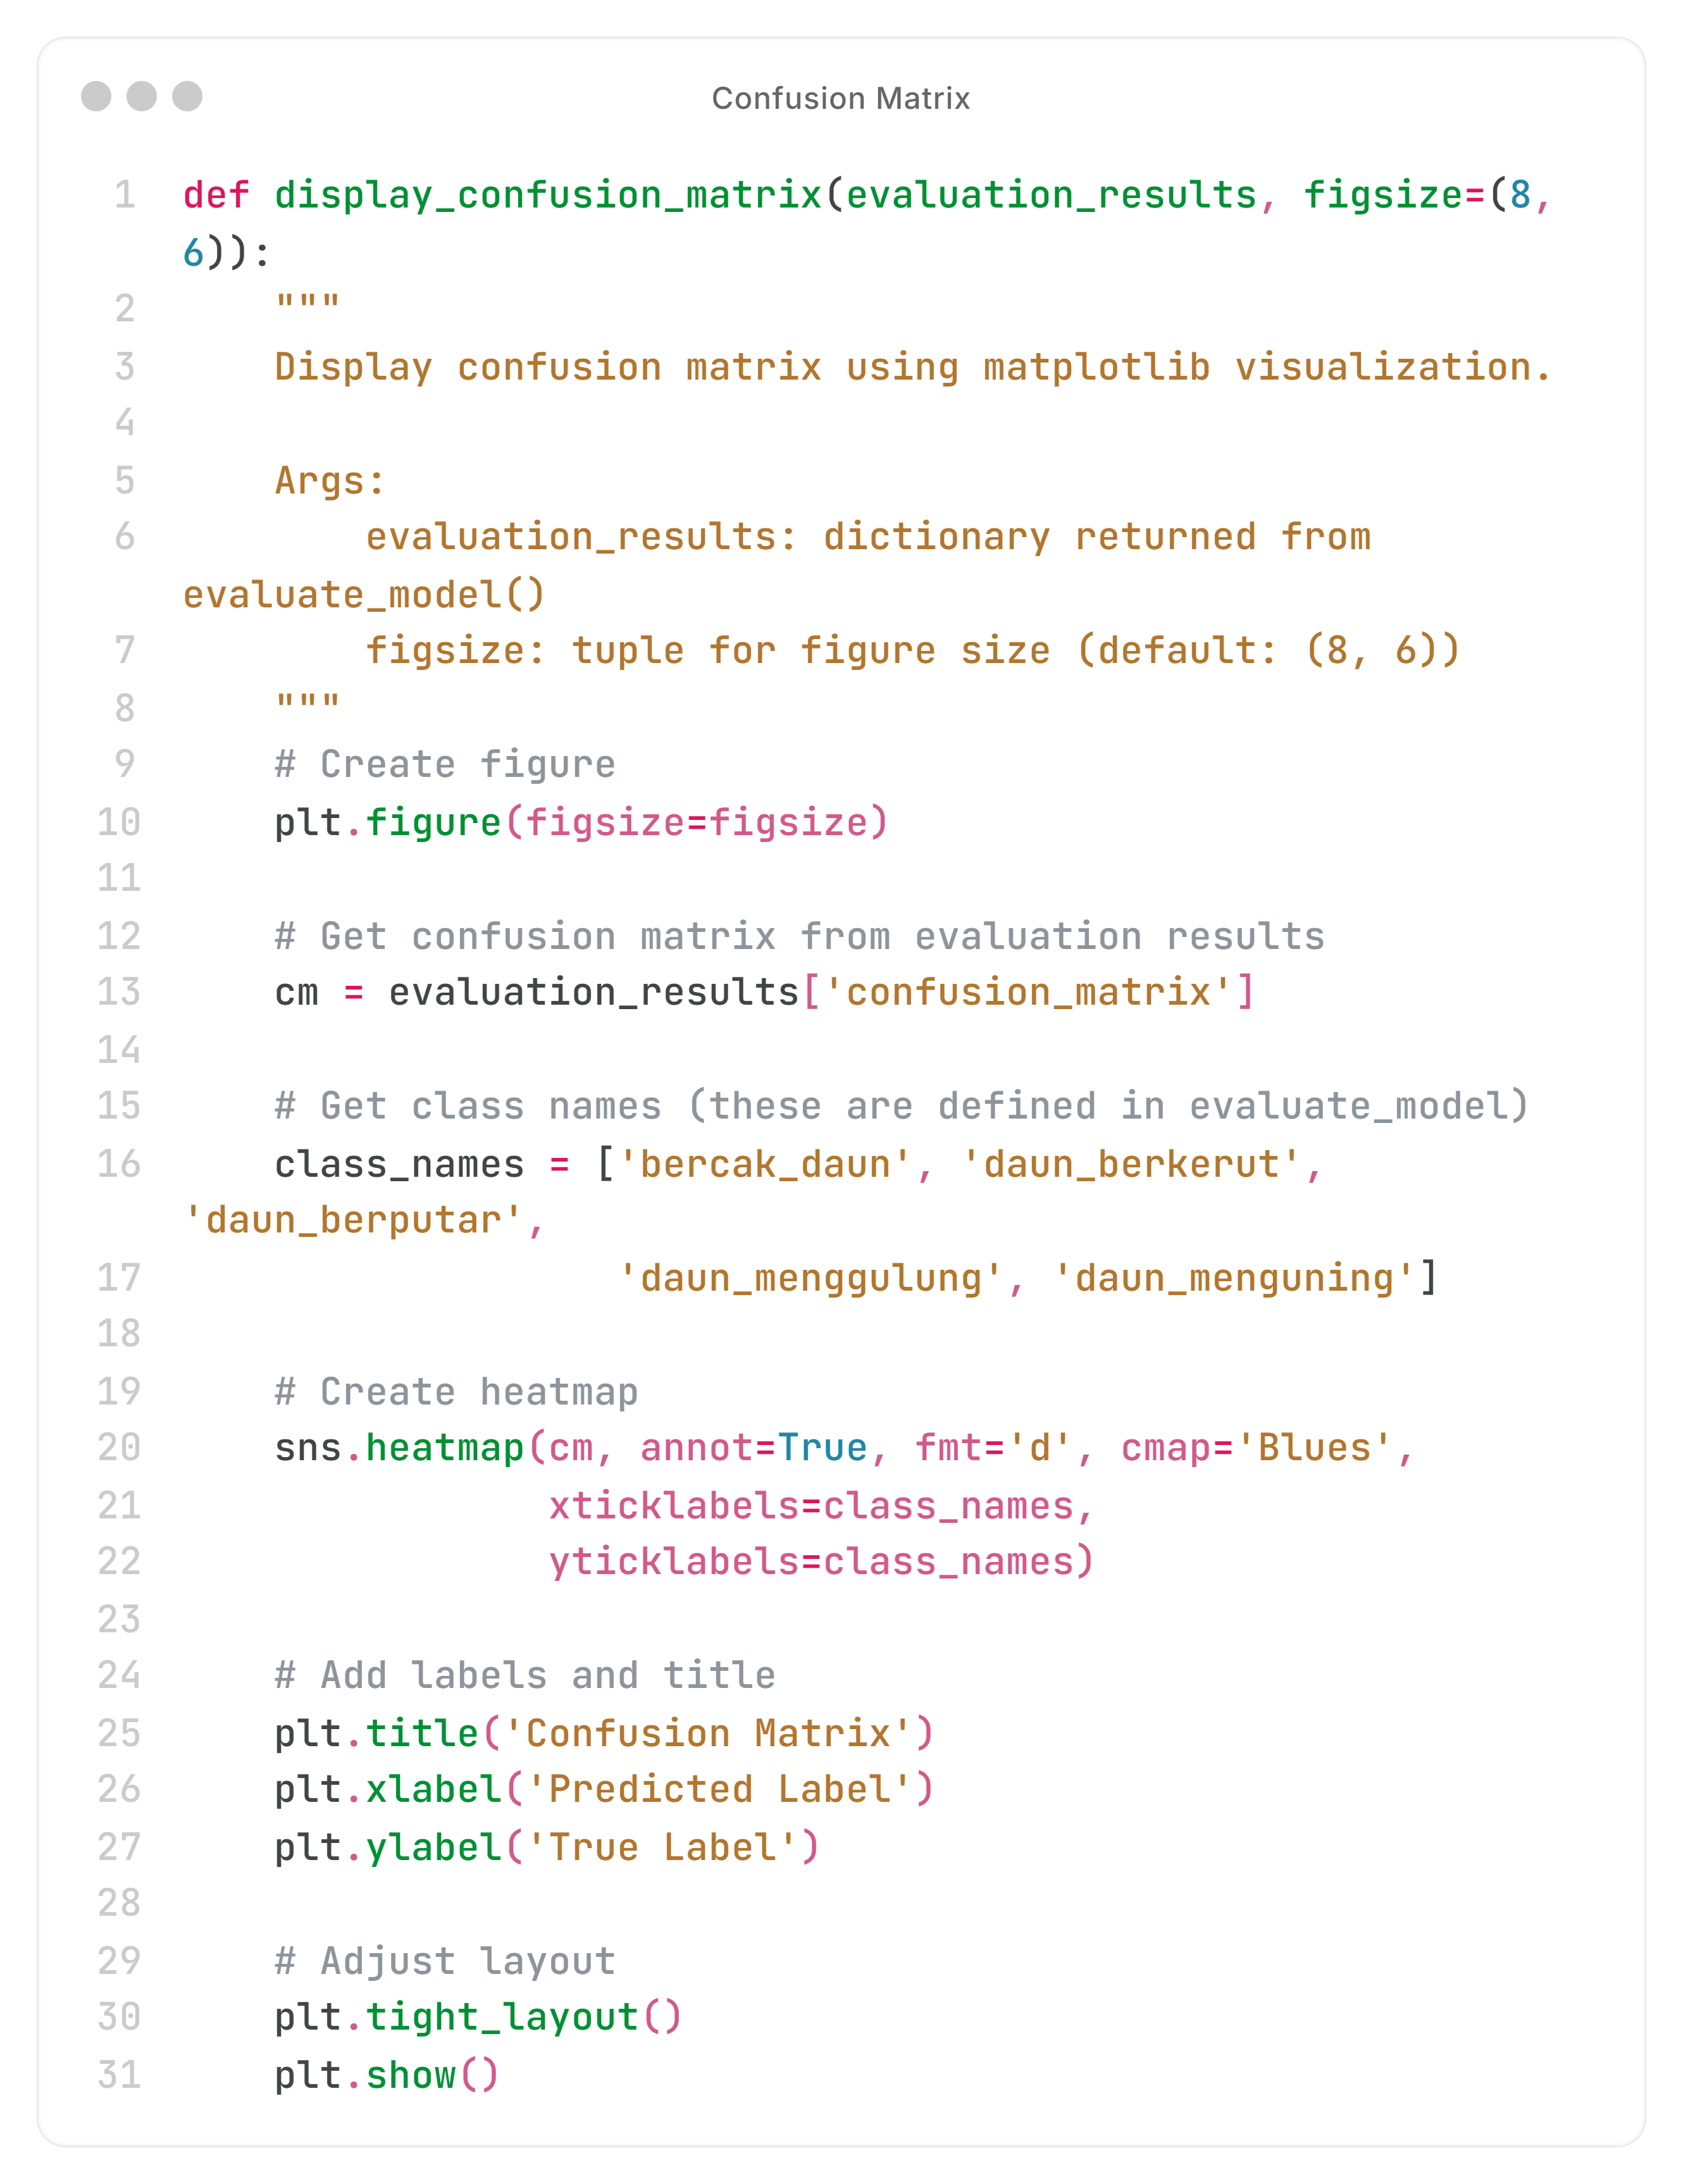
\includegraphics[width=0.6\textwidth]{figure/chapter-4-confusion.png}
  \caption{Contoh hasil confusion matrix}
  \label{fig:extract_rgb}
\end{figure}

Fungsi ini memvisualisasikan hasil prediksi dalam bentuk \textit{heatmap}, sehingga mempermudah analisis kesalahan klasifikasi antar kelas.

\begin{figure}[H]
  \centering
  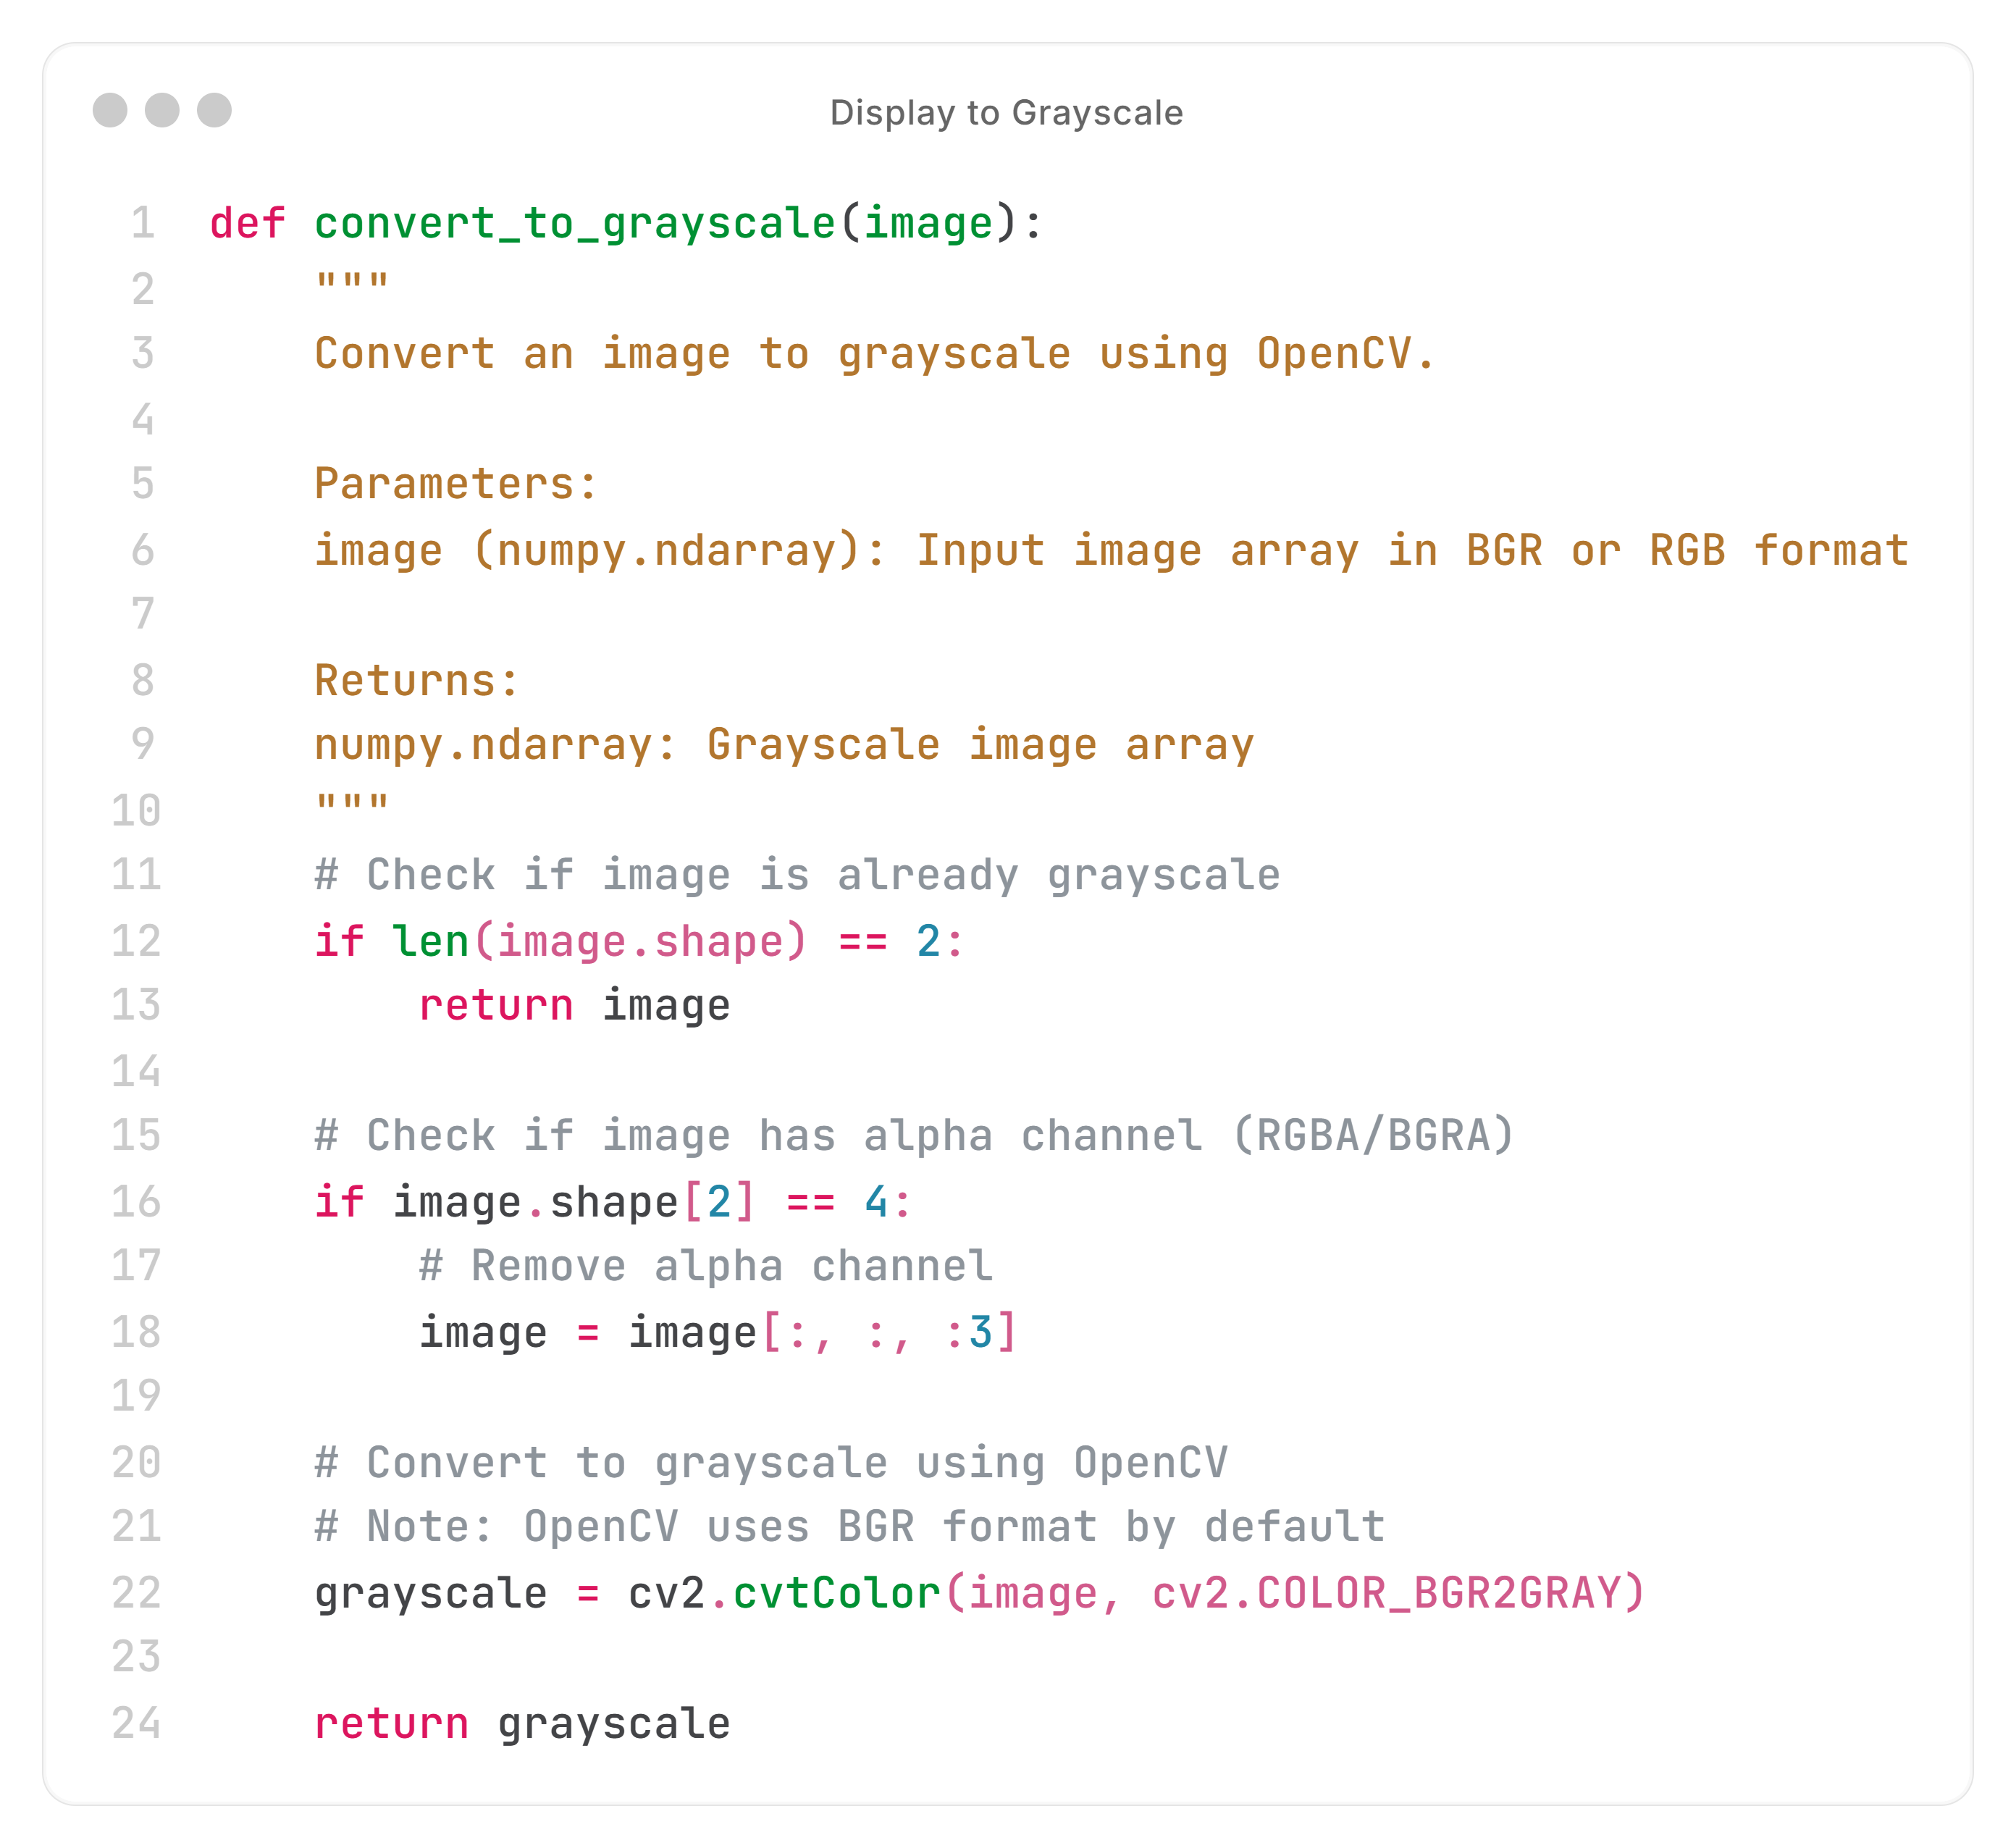
\includegraphics[width=0.6\textwidth]{figure/chapter-4-convert_to_grayscale.png}
  \caption{Contoh hasil konversi citra daun ke grayscale}
  \label{fig:extract_rgb}
\end{figure}

\begin{figure}[H]
  \centering
  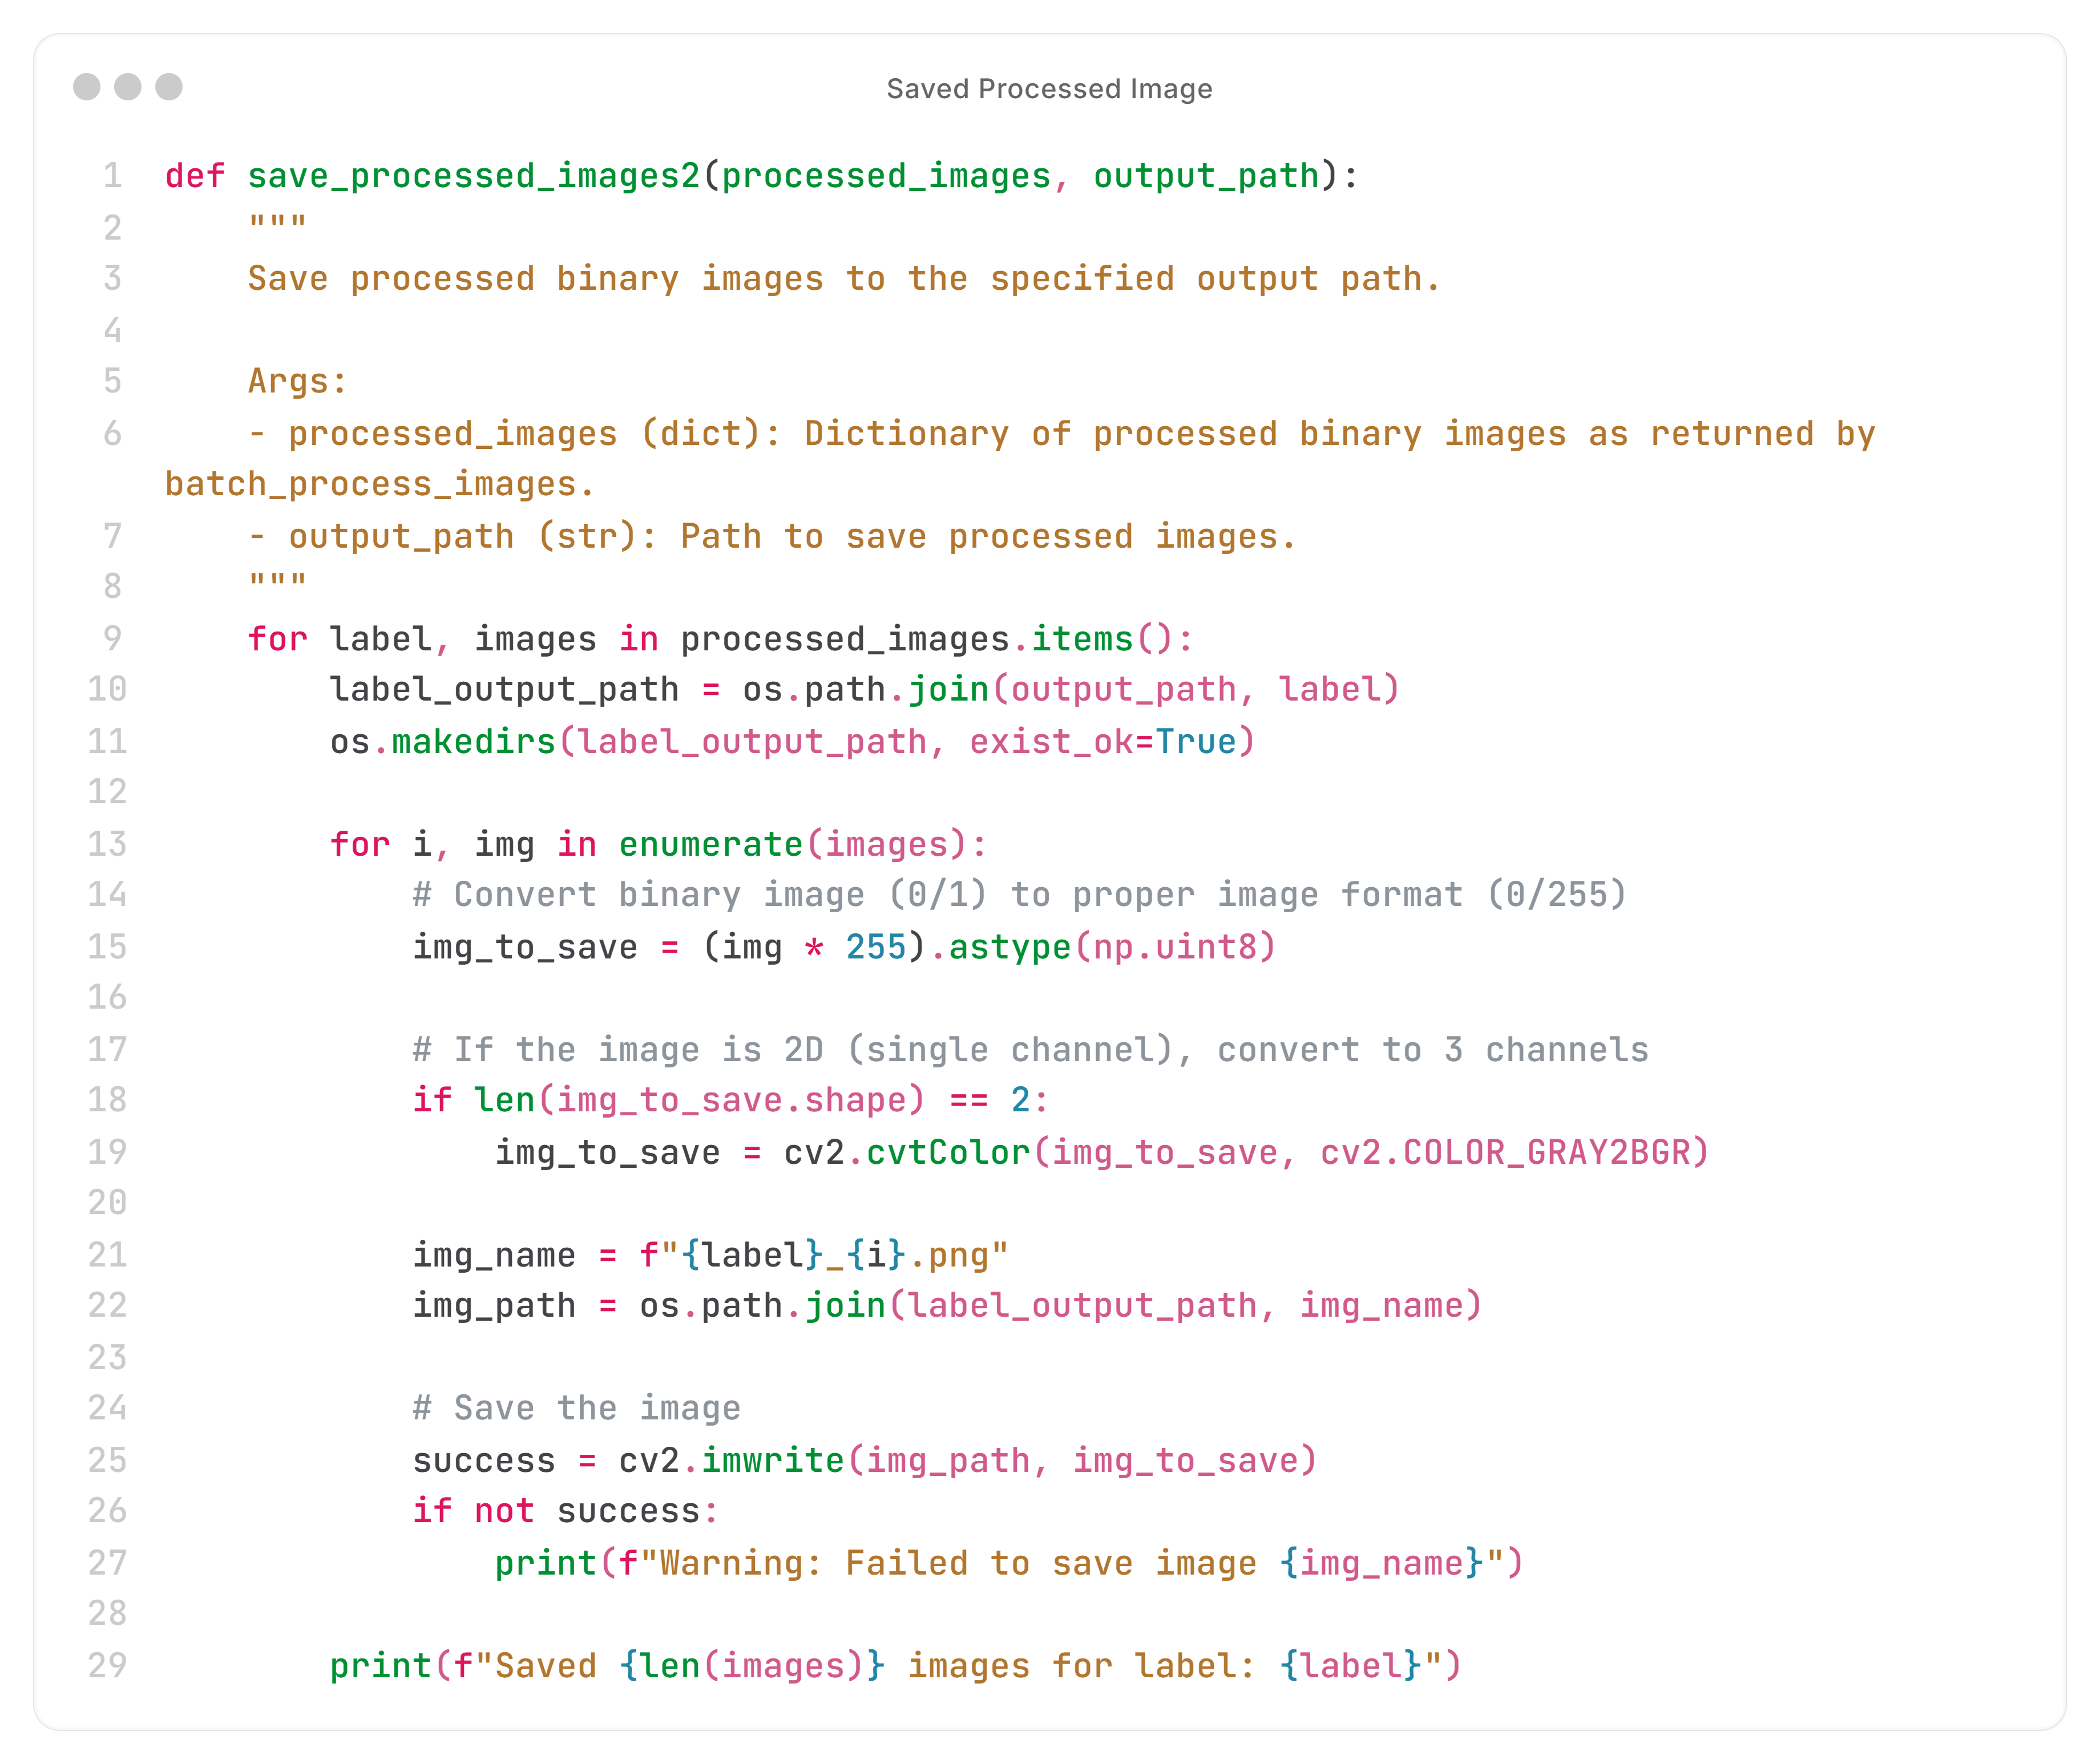
\includegraphics[width=0.6\textwidth]{figure/chapter-4-save_processed_images2.png}
  \caption{Contoh hasil pemrosesan gambar daun menjadi kerangka data}
  \label{fig:extract_rgb}
\end{figure}

\begin{figure}[H]
  \centering
  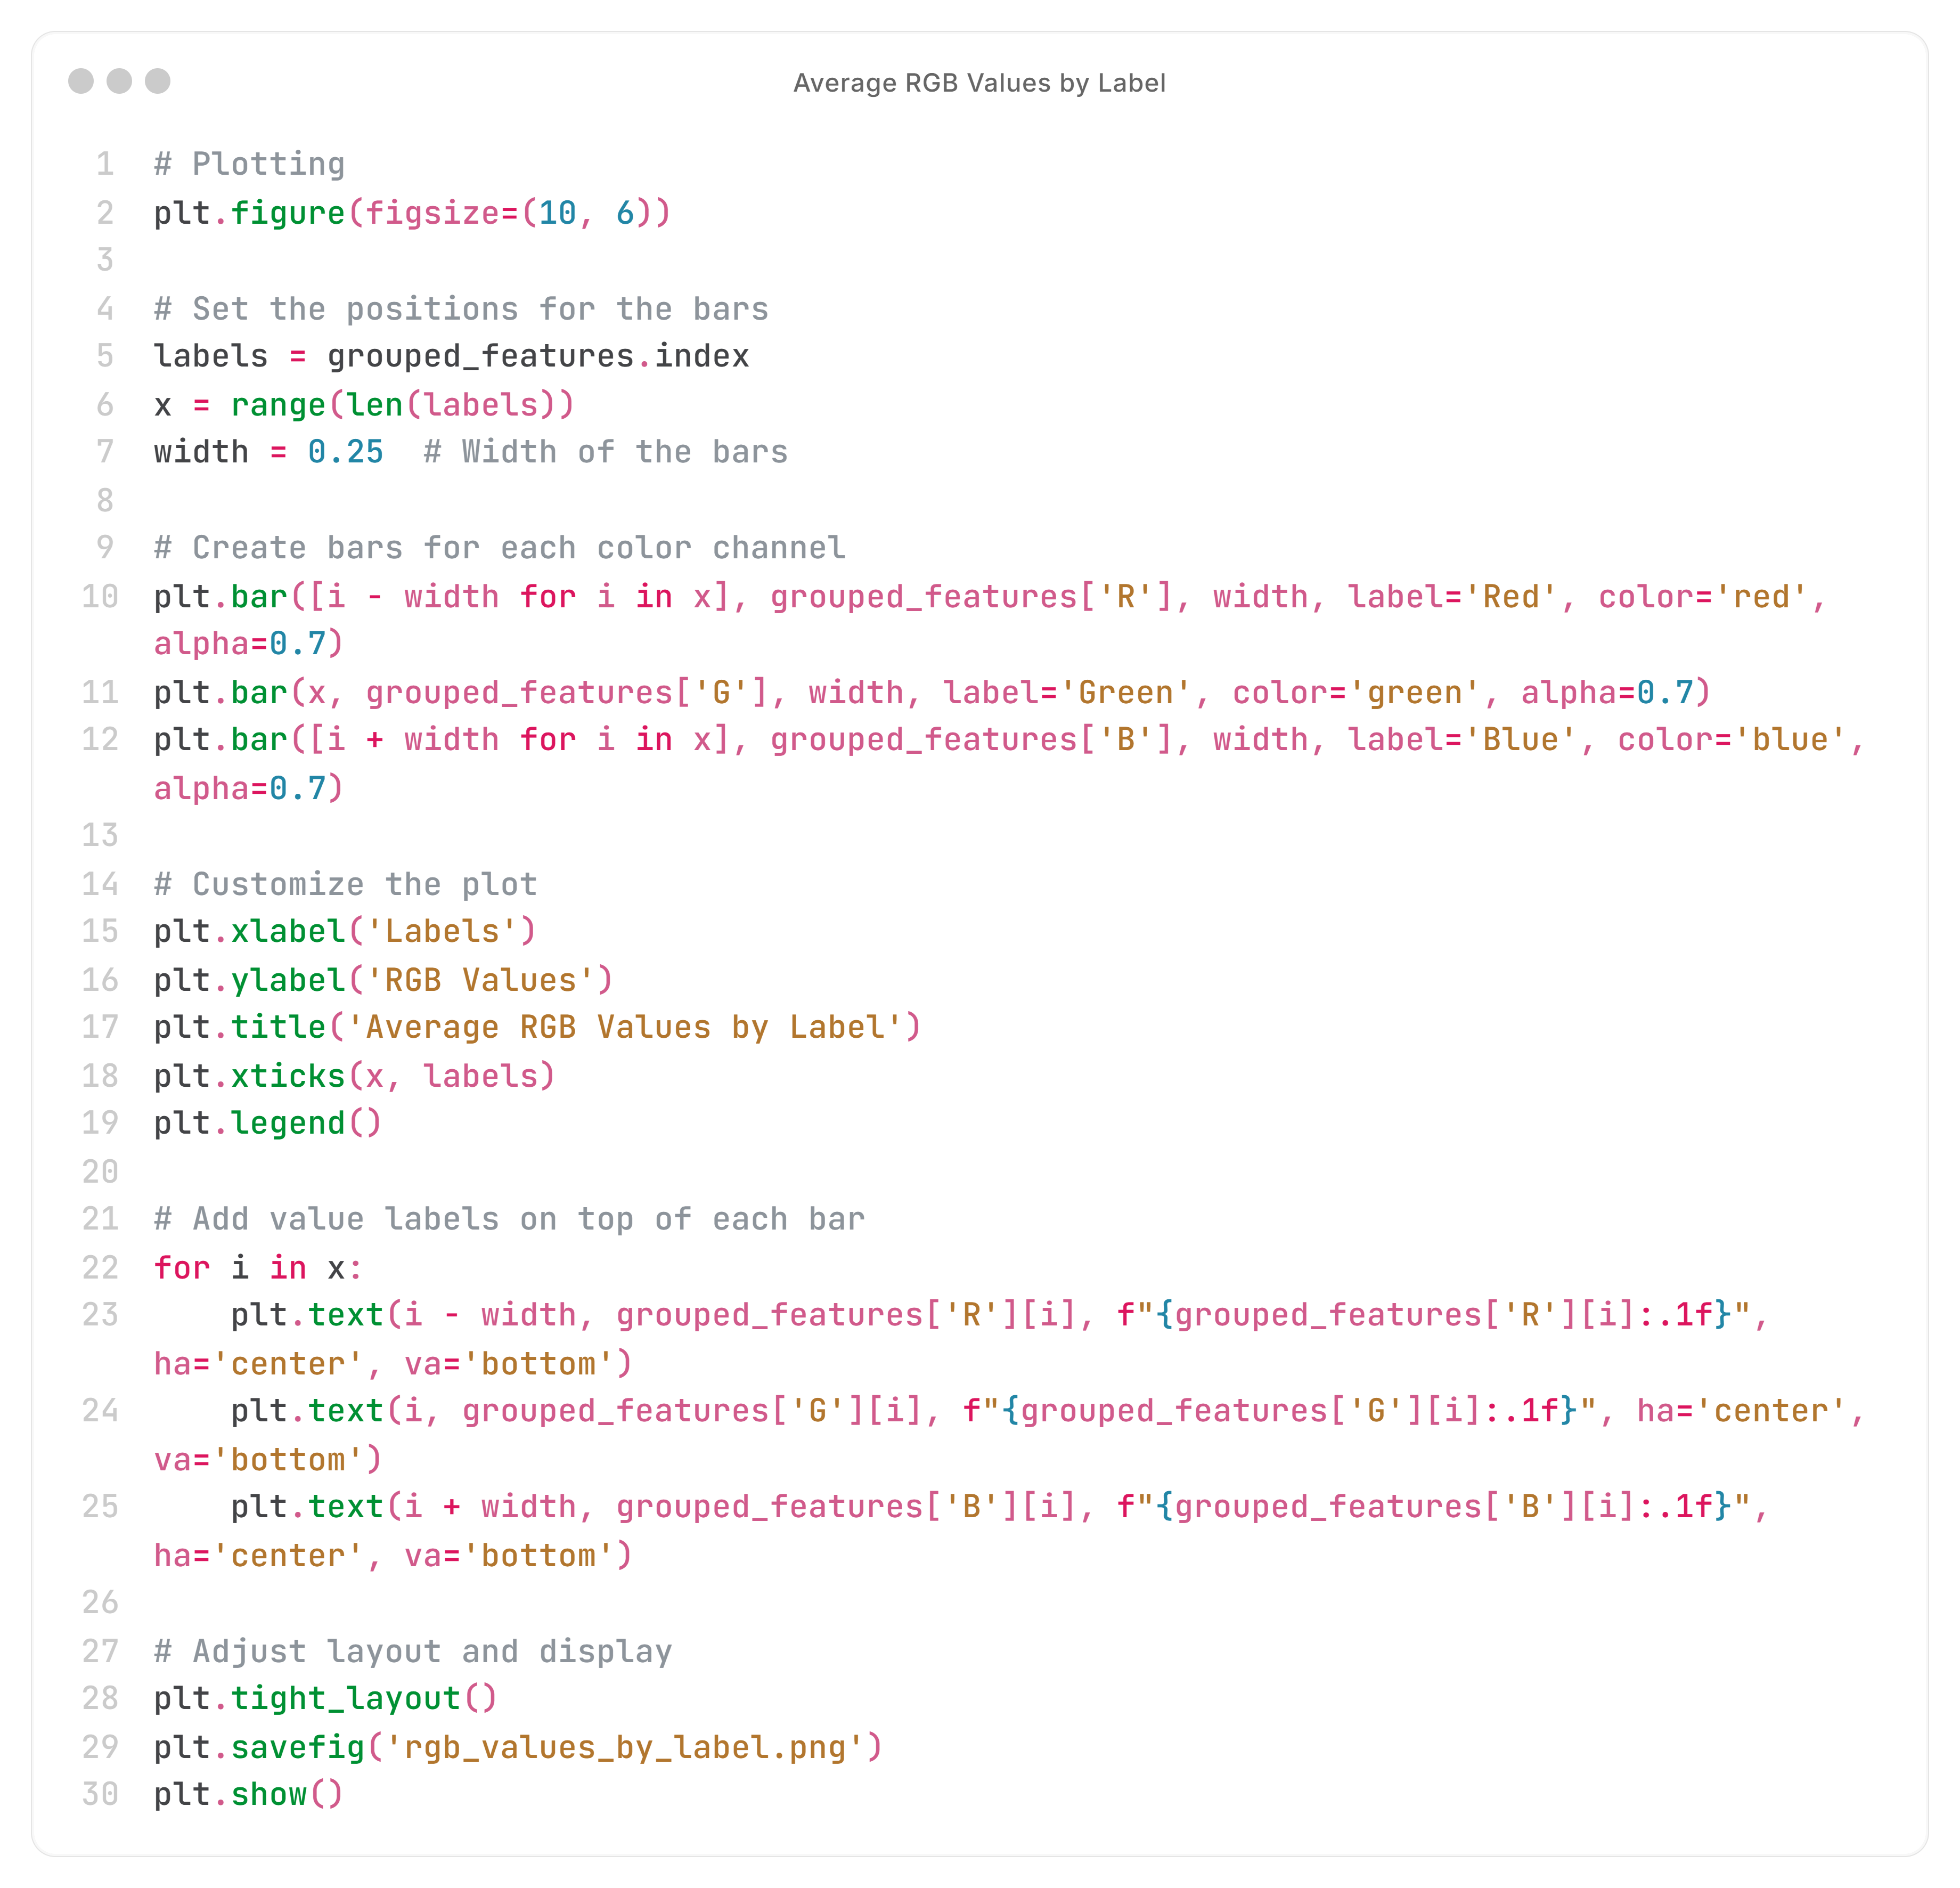
\includegraphics[width=0.6\textwidth]{figure/chapter-4-average_rgb.png}
  \caption{Contoh hasil rata-rata RGB dari citra daun}
  \label{fig:extract_rgb}
\end{figure}

\begin{figure}[H]
  \centering
  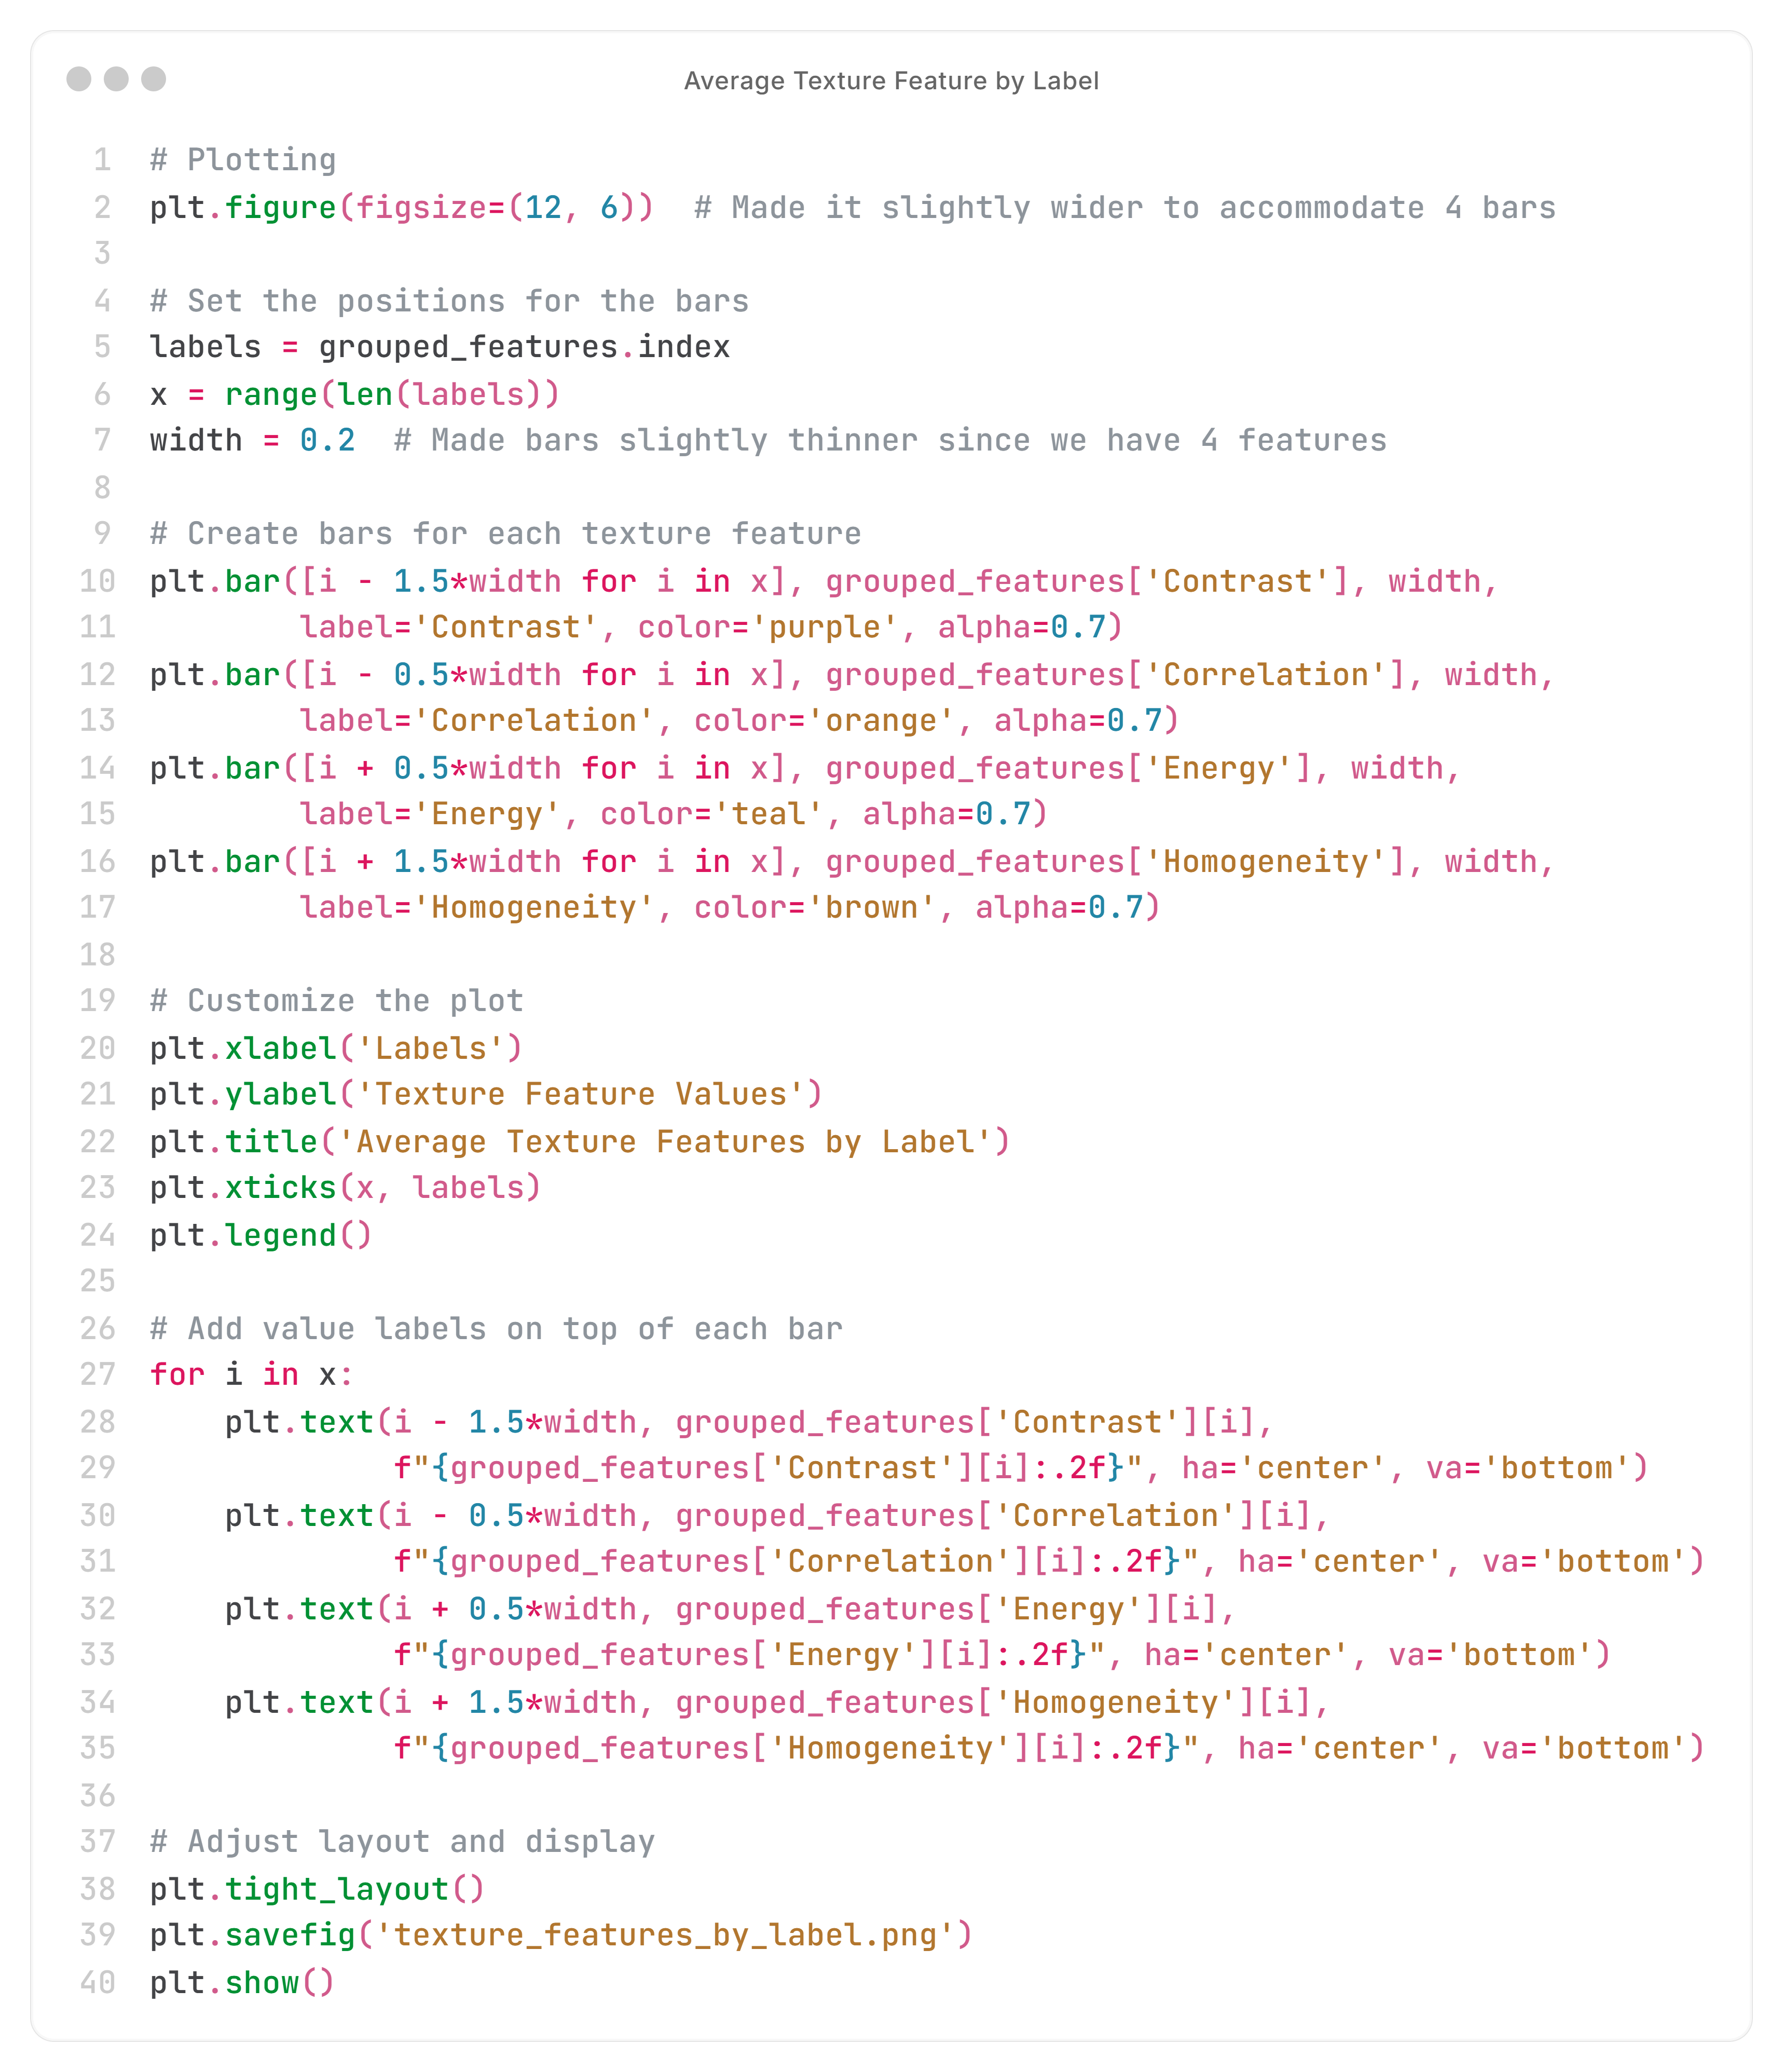
\includegraphics[width=0.6\textwidth]{figure/chapter-4-average_texture.png}
  \caption{Contoh hasil rata rata ekstraksi fitur tekstur}
  \label{fig:extract_rgb}
\end{figure}

\begin{figure}[H]
  \centering
  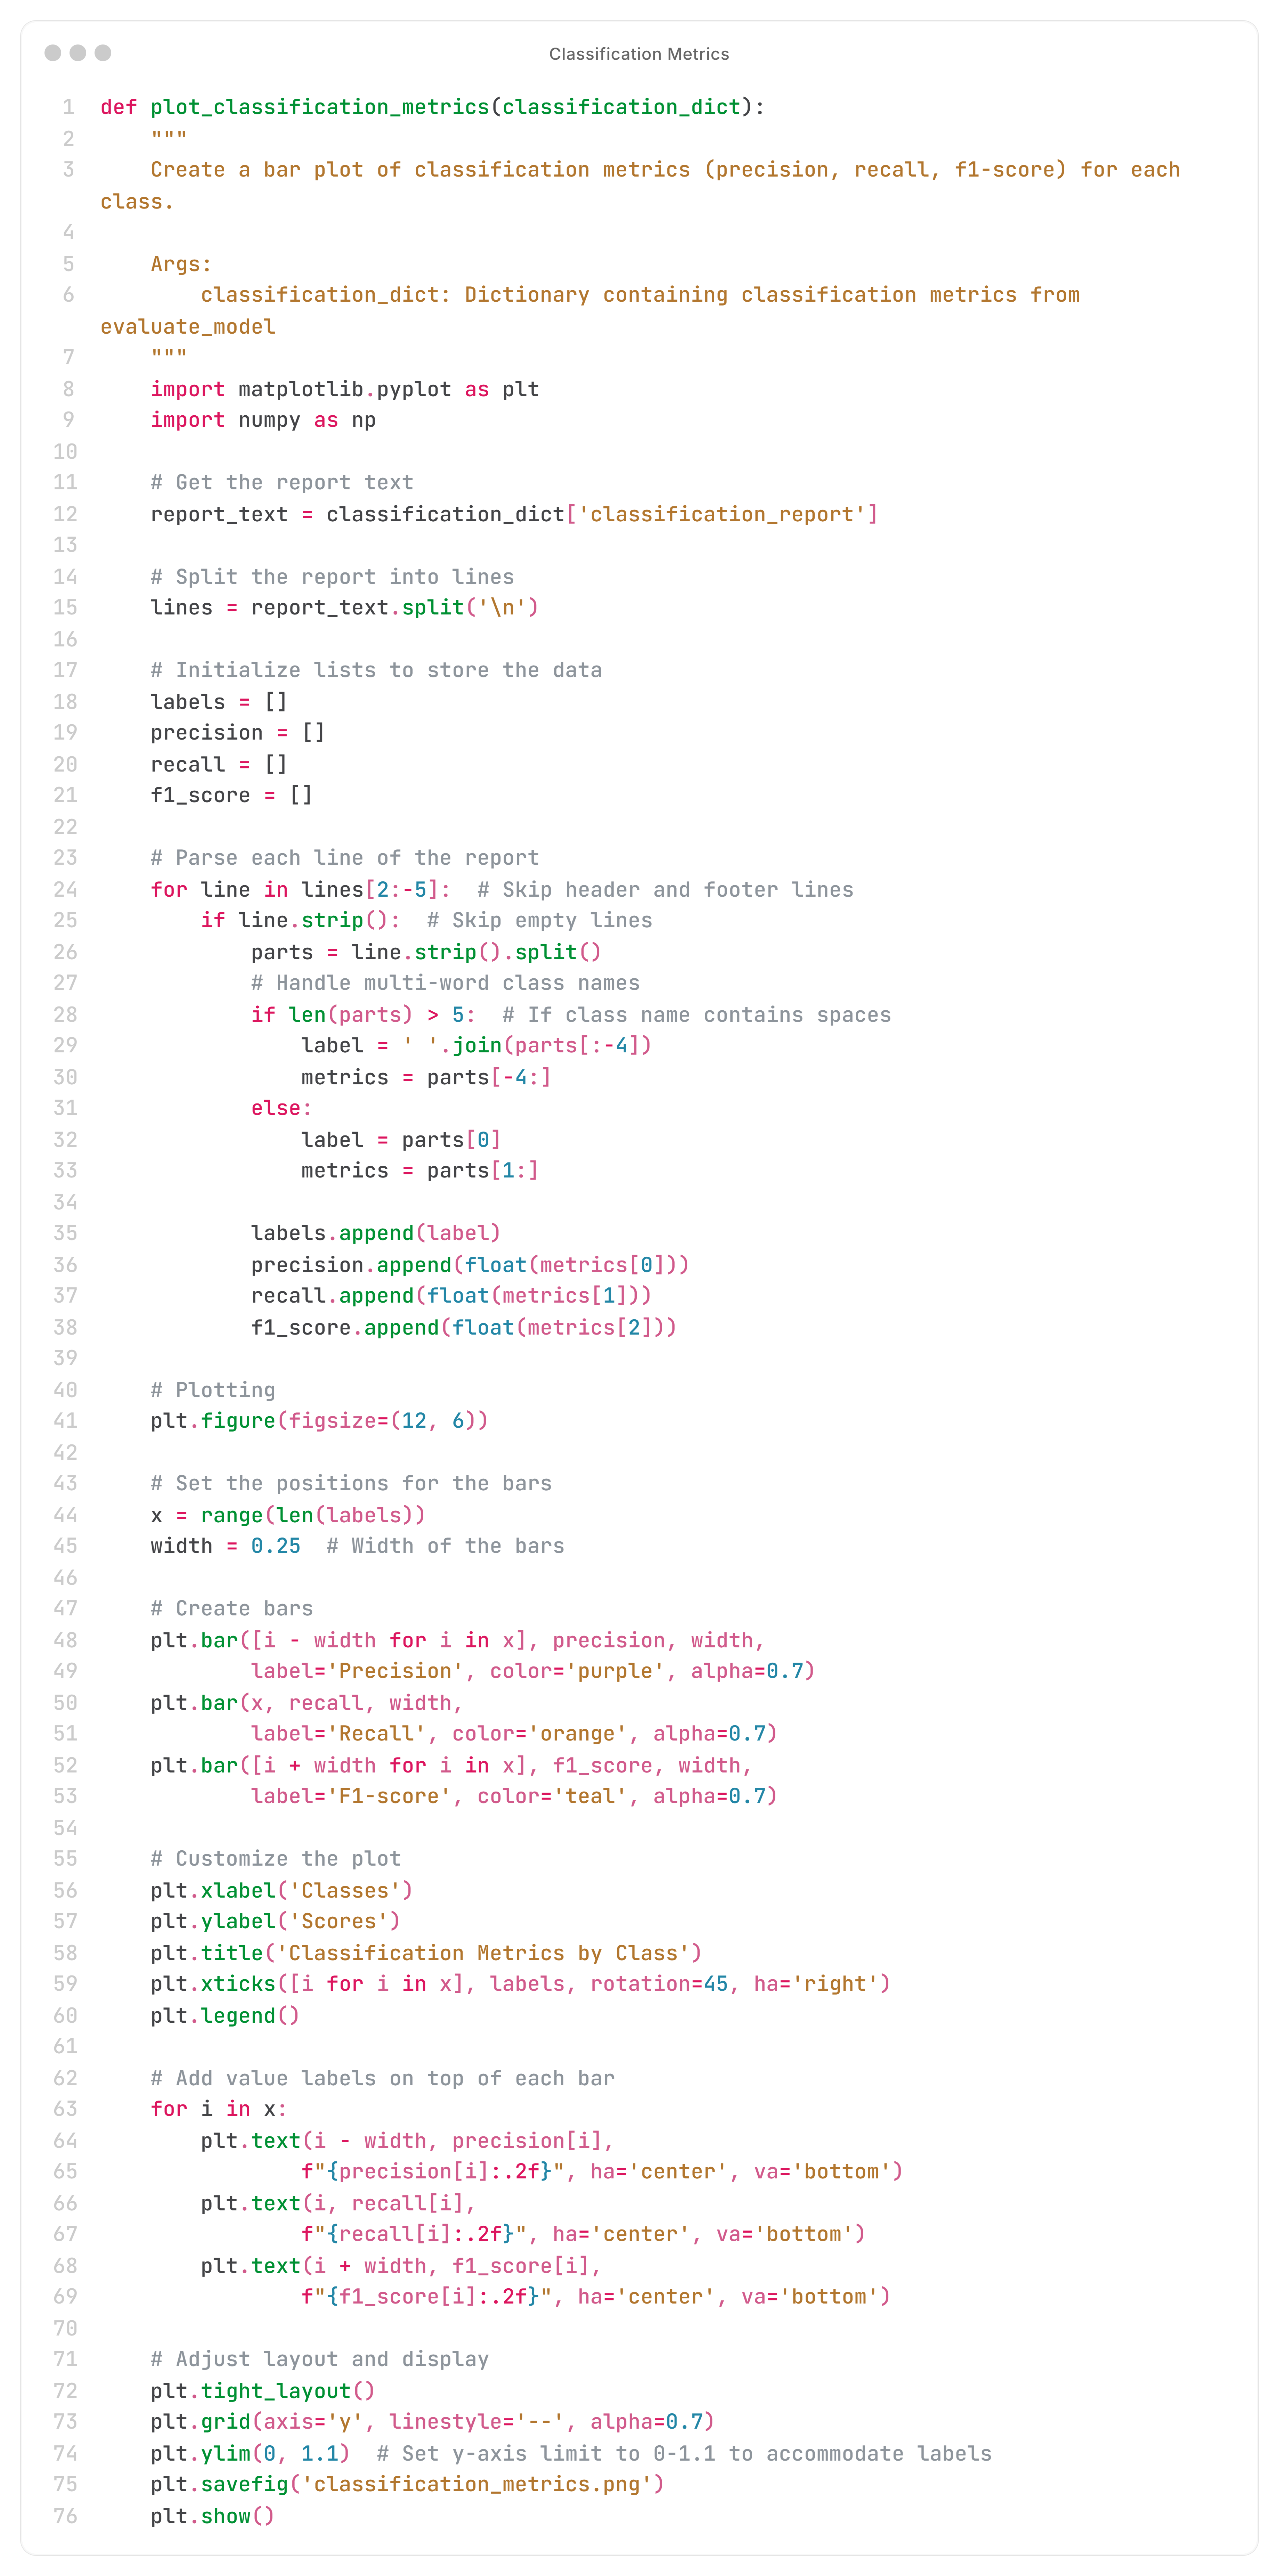
\includegraphics[width=0.6\textwidth]{figure/chapter-4-classification_metrics.png}
  \caption{Contoh hasil classification metrics}
  \label{fig:extract_rgb}
\end{figure}